\documentclass[letterpaper]{article} % DO NOT CHANGE THIS
\usepackage[submission]{aaai2027} % DO NOT CHANGE THIS
\usepackage[hyphens]{url} % DO NOT CHANGE THIS
\usepackage{graphicx} % DO NOT CHANGE THIS
\urlstyle{rm} % DO NOT CHANGE THIS
\def\UrlFont{\rm} % DO NOT CHANGE THIS
\usepackage{natbib} % DO NOT CHANGE THIS AND DO NOT ADD OPTIONS
\usepackage{caption} % DO NOT CHANGE THIS AND DO NOT ADD OPTIONS
\frenchspacing % DO NOT CHANGE THIS
\setlength{\pdfpagewidth}{8.5in} % DO NOT CHANGE THIS
\setlength{\pdfpageheight}{11in} % DO NOT CHANGE THIS

\usepackage{amsmath}
\usepackage{amssymb}
\usepackage{amsthm}
\usepackage{booktabs}
\usepackage{array}
\usepackage{multirow}
\usepackage{xspace}
\usepackage{algorithm}
\usepackage{algorithmic}

\setcounter{secnumdepth}{2}
\graphicspath{{figures/}}

\newcommand{\method}{\textup{\textsc{E2E-Merge}}\xspace}
\newcommand{\norm}[1]{\left\lVert #1\right\rVert}
\newcommand{\R}{\mathbb R}

\theoremstyle{plain}
\newtheorem{theorem}{Theorem}
\newtheorem{proposition}[theorem]{Proposition}
\newtheorem{lemma}[theorem]{Lemma}
\newtheorem{corollary}[theorem]{Corollary}
\theoremstyle{definition}
\newtheorem{assumption}[theorem]{Assumption}
\newtheorem{remark}[theorem]{Remark}

\pdfinfo{
/TemplateVersion (2027.1)
}

\title{Model Consolidation under Budget:\\
From Closed-Form Merging to End-to-End Distillation}
\author{Anonymous Submission}
\affiliations{}

\begin{document}
\maketitle

\begin{abstract}
Data-assisted model consolidation is commonly approached in two computational regimes: closed-form merging, which cheaply solves parameter-space or layer-local surrogates, and multi-teacher distillation, which spends iterative computation to match expert behavior end to end.
We study when each regime is preferable rather than treating one as universally superior.
Both are organized around a task-conditioned functional objective: on inputs from task $a$, one shared model should reproduce expert $a$.
Our analysis separates the fixed \emph{surrogate gap} of closed-form regression from the data- and compute-dependent errors of end-to-end distillation.
Locally, RegMean is the exact optimizer of an expert-centered, layer-wise, first-order, isotropic surrogate; dropping cross-layer coupling incurs an exact quadratic excess loss.
Under local smoothness and Polyak--Lojasiewicz conditions, iterative refinement reduces the original functional error with computation and admits a sufficient break-even budget.
A finite-data bound gives the complementary condition under which the estimation and optimization errors of distillation fall below a closed-form reference.
We also show that logit distillation uses a task-head-induced semimetric, whereas representation matching supervises the full shared representation.
Existing experiments map three slices of the resulting frontier without introducing new measurements.
On ViT-B/32, RegMean++ is better with only $64$--$128$ distinct examples per task, while representation distillation overtakes it at $256$ and above; $4$k, $8$k, and $12$k updates reach $89.2\%$, $90.1\%$, and $90.2\%$ versus $84.2\%$ for RegMean++; and block-wise refinement spans $85.3\%$ at $3.7$ GB to $89.8\%$ at $5.4$ GB before the full $90.2\%$ endpoint.
The distillation advantage grows with expert count and weaker backbones, whereas a preliminary Flan-T5 GLUE probe, using different functional readouts, favors closed-form RegMean.
The evidence supports a regime view: closed-form merging is preferable under severe data, compute, or memory constraints and when its surrogate is tight; end-to-end distillation pays when sufficient unlabeled data and offline computation are available and the structural gap is large.
\end{abstract}

\section{Introduction}
\label{sec:intro}

Model consolidation turns several task experts derived from a common checkpoint into one model with the original architecture and inference cost.
The literature is often described as a collection of merging algorithms, but data-assisted methods now occupy two visibly different computational regimes.
At one end, closed-form methods such as Fisher merging, RegMean, and RegMean++ collect a small set of statistics and solve a parameter- or layer-local problem once \citep{matena2022fisher,jin2023regmean,regmeanplusplus2025}.
At the other end, optimization-based mergers and multi-teacher distillation repeatedly query the experts and update a student on unlabeled inputs \citep{yang2024adamerging,prodistill2025,samerging2025}.
Both return a single consolidated model, but they trade accuracy, data, computation, and memory differently.

This paper asks a broader question than whether one particular method wins at its most accurate operating point:
\begin{quote}
\emph{When does a cheap closed-form merge suffice, and when is the additional cost of end-to-end distillation justified?}
\end{quote}
The answer cannot be reduced to accuracy divided by wall-clock time.
A practitioner may be limited by distinct unlabeled examples, student backward passes, peak activation memory, or the number and incompatibility of experts.
Moreover, the two regimes make different kinds of error.
A closed-form method can exactly solve its chosen surrogate yet remain biased for the deployed end-to-end function.
Distillation attacks that function more directly, but its finite-data and optimization errors can be large when data or iterations are scarce.

We organize both regimes around the same ideal task-conditioned functional objective.
Let $g_{\theta_a}$ be expert $a$, and let $\mathcal D_a$ be its unlabeled input distribution.
A consolidated model should reproduce expert $a$ on inputs from task $a$:
\begin{equation}
F(\theta)=\sum_{a=1}^{T}\pi_a
\mathbb E_{X\sim\mathcal D_a}
\left[\|g_\theta(X)-g_{\theta_a}(X)\|_2^2\right].
\label{eq:functional-objective}
\end{equation}
Task-conditioned multi-teacher distillation samples this objective directly.
Closed-form mergers approximate it.
In particular, RegMean is not a logit method: it performs closed-form regression on each linear layer's activations or outputs.
We show that it is the exact optimizer of an expert-centered, layer-wise, first-order surrogate after the downstream metric is replaced by a shared isotropic one.
This explains why RegMean is strong and why it may retain a fixed gap when downstream anisotropy, cross-layer coupling, merged-model activations, or nonlinear re-linearization matter.

The same framework also separates \emph{what is distilled} from \emph{how it is optimized}.
CLIP tasks use different class sets and text-prototype heads.
Logit or KL matching sees a representation only through the current head, whereas representation matching supervises a shared, head-independent space.
We characterize the exact spectral condition under which all observed heads jointly control the full representation.

The theory leads to a budgeted regime condition.
A closed-form reference has a structural functional gap $\Delta_{\mathrm{CF}}$.
End-to-end distillation with $n$ distinct examples and $K$ updates has finite-data and optimization terms.
Under a standard uniform-deviation condition, a sufficient comparison takes the form
\begin{equation}
\underbrace{2\varepsilon_n+\delta_K}_{\text{distillation: data + optimization}}
<
\underbrace{\Delta_{\mathrm{CF}}}_{\text{closed-form structural gap}},
\label{eq:regime-condition}
\end{equation}
where $\varepsilon_n$ is the empirical-to-population deviation and $\delta_K$ is empirical optimization error.
Locally, $\Delta_{\mathrm{CF}}$ is quantified by exact normal-equation, subspace, and cross-layer gap formulas; under local smoothness and a Polyak--Lojasiewicz condition, $\delta_K$ decreases geometrically in an idealized analysis.
Equation \eqref{eq:regime-condition} is not a claim that distillation always wins.
It predicts a crossover in data and computation, and it predicts that the crossover should move in favor of distillation as the closed-form surrogate becomes less accurate.

The existing experiments already expose these regimes.
On ViT-B/32, RegMean++ leads with only $64$ or $128$ distinct examples per task, but representation distillation overtakes it at $256$ and widens the gap thereafter.
Along the selected learning-rate trajectory, $4$k updates recover $83.3\%$ of the final measured gain over RegMean++, $8$k recover $98.3\%$, and the final $4$k add only $0.1$ point.
Block-wise refinement gives intermediate memory--accuracy operating points.
The gain over closed-form merging grows from $2.6$ points at two experts to $6.0$ at eight and $13.7$ at twenty on ViT-B/32, and is larger on weaker backbones for the same twenty tasks.
Conversely, the preliminary Flan-T5 GLUE probe favors closed-form RegMean ($83.0\%$) over iterative distillation ($81.9\%$), under the caveat that the two use different functional readouts.
These are precisely the kinds of crossovers a regime analysis should explain.

\paragraph{Contributions.}
\begin{itemize}
    \item We formulate closed-form merging and end-to-end distillation as two
computational regimes of task-conditioned functional consolidation.
A Bayes decomposition and a margin bound connect the objective to expert preservation.
    \item We derive an approximation--estimation--optimization view of method choice.
Exact local formulas quantify normal-equation mismatch, restricted update subspaces, and omitted cross-layer coupling; a finite-data bound and a compute-dependent descent result give sufficient break-even conditions.
    \item We distinguish target coverage from solver choice. The aggregate task heads
define a positive-semidefinite frame operator; logit supervision is equivalent to representation supervision only when it has a positive lower frame bound.
    \item Using only existing measurements, we reorganize the empirical study around
data, iteration, memory, and consolidation-difficulty frontiers.
The resulting regime map identifies where closed-form merging, block-wise refinement, and full end-to-end distillation are preferable within the studied settings.
\end{itemize}

\section{Related Work}
\label{sec:related}

\paragraph{Closed-form and parameter-space merging.}
Model soups and task arithmetic combine parameters directly \citep{wortsman2022modelsoups,ilharco2023taskarithmetic}.
TIES and DARE edit signs and sparsity \citep{yadav2023ties,yu2024dare}; TSV-M and Iso-C use task-vector subspaces \citep{gargiulo2025tsvm,marczak2025isotropic}; Fisher merging uses a diagonal sensitivity metric \citep{matena2022fisher}.
RegMean fits each linear layer by closed-form regression, and RegMean++ improves the layer inputs by propagating the partially merged network \citep{jin2023regmean,regmeanplusplus2025}.
FeatCal and Output-Space Projection further emphasize feature- or output-space calibration with efficient local solvers \citep{featcal2026,outputprojection2026}.
These methods occupy low-compute operating points, but differ in the target and local geometry they retain.

\paragraph{Optimization and distillation.}
AdaMerging optimizes merge coefficients on unlabeled data \citep{yang2024adamerging}.
ProDistill performs progressive layer-wise distillation, while SAMerging formulates merging as multi-teacher logit distillation with sharpness-aware optimization \citep{prodistill2025,samerging2025}.
Classical knowledge distillation provides the general teacher--student framework \citep{hinton2015distilling}.
Our focus is not priority for using distillation.
We compare the computational regimes and characterize when the extra optimization can overcome the structural gap of a closed-form surrogate.

\paragraph{Representations and inference-time modules.}
Representation Surgery and weight-ensembling mixtures introduce feature corrections or routing at inference \citep{yang2024surgery,tang2024wemoe}.
The setting here instead returns one shared encoder with no learned router or task-specific trainable module; evaluation still chooses each task's fixed CLIP class set and text-prototype head.

\section{A Budgeted Functional View}
\label{sec:theory}

\subsection{One functional objective, two computational regimes}
\label{sec:common-objective}

Let $A$ be a task with probability $\pi_a$, draw $X\mid A=a\sim\mathcal D_a$, and set $Z=g_{\theta_A}(X)$.
Equation~\eqref{eq:functional-objective} is equivalently $F(\theta)=\mathbb E\|g_\theta(X)-Z\|_2^2$.
Its unconstrained Bayes target is $\mu(x)=\mathbb E[Z\mid X=x]$, and
\begin{equation}
F(h)=\mathbb E\|h(X)-\mu(X)\|_2^2
+\mathbb E\|Z-\mu(X)\|_2^2.
\label{eq:bayes-main}
\end{equation}
The second term is irreducible conflict among experts on overlapping inputs.
The first is what a shared model can reduce.
A margin argument further gives, for every $\gamma_0>0$,
\begin{equation}
|\mathrm{Acc}_a(\theta)-\mathrm{Acc}_a(\theta_a)|
\le
\Pr[\gamma_a(X)\le\gamma_0]
+\frac{4F_a(\theta)}{\gamma_0^2},
\label{eq:accuracy-main}
\end{equation}
where $F_a$ is task $a$'s representation loss and $\gamma_a$ is the expert top-two margin.
Thus the functional discrepancy is aligned with preserving the experts, though it is not identical to ground-truth accuracy.

Closed-form and iterative methods address Eq.~\eqref{eq:functional-objective} differently.
A closed-form method selects a surrogate $\widetilde F$ that can be solved analytically or with a small linear system.
Its optimization error on $\widetilde F$ is negligible, but its output can retain a structural gap on $F$.
Distillation uses samples of $F$ itself, but must estimate and optimize it.
This yields the schematic comparison
\begin{equation}
\begin{aligned}
\mathcal E_{\mathrm{CF}}(n)
&\approx \Delta_{\mathrm{sur}}+\Delta_{\mathrm{est}}^{\mathrm{CF}}(n),\\
\mathcal E_{\mathrm{Dist}}(n,K)
&\approx \Delta_{\mathrm{est}}^{\mathrm{Dist}}(n)
+\Delta_{\mathrm{opt}}(K).
\end{aligned}
\label{eq:schematic-errors}
\end{equation}
Equation~\eqref{eq:schematic-errors} is an organizing decomposition, not an exact equality for arbitrary neural networks.
The next results make its structural and optimization parts precise under local assumptions.

\subsection{The fixed structural gap of closed-form regression}
\label{sec:closed-form-gap}

Around a reference merge $\bar\theta$, linearize the residual and add damping:
\begin{equation}
Q(\Delta)=C-b^\top\Delta+\tfrac12\Delta^\top H\Delta,
\qquad H\succ0.
\label{eq:local-quadratic}
\end{equation}
The full local optimum is $\Delta^\star=H^{-1}b$.
For any surrogate update $\widetilde\Delta$,
\begin{equation}
Q(\widetilde\Delta)-Q(\Delta^\star)
=\tfrac12\|H\widetilde\Delta-b\|_{H^{-1}}^2.
\label{eq:gap-main}
\end{equation}
If the surrogate solves $\widetilde H\widetilde\Delta=\widetilde b$, the residual becomes $(H-\widetilde H)\widetilde\Delta+(\widetilde b-b)$, separating geometry from trajectory/target mismatch.
If $H=D+E$ and a layer-wise method keeps only the block diagonal $D$, its exact local excess is
\begin{equation}
Q(\Delta_D)-Q(\Delta^\star)
=\tfrac12\|E\Delta_D\|_{H^{-1}}^2,
\qquad \Delta_D=D^{-1}b.
\label{eq:cross-layer-gap-main}
\end{equation}
Likewise, restricting updates to $\Delta=Uc$ for a coefficient vector $c$ loses the $H$-energy of the unrestricted solution outside $\operatorname{col}(U)$.

\begin{proposition}[Local structural gap]
\label{prop:local-gap-main}
Let $Q$ be given by Eq.~\eqref{eq:local-quadratic}.
If a surrogate returns $\widetilde\Delta$ by solving $\widetilde H\widetilde\Delta=\widetilde b$, then its excess local functional loss is exactly \[ \frac12\left\|(H-\widetilde H)\widetilde\Delta+(\widetilde b-b)\right\|_{H^{-1}}^2.
\] For a block-diagonal approximation $D$ this reduces to $\tfrac12\|E\Delta_D\|_{H^{-1}}^2$, and for a restricted subspace it equals the $H$-energy of the full update outside that subspace.
\end{proposition}

The proposition separates three quantities that are otherwise conflated in a method-level comparison: the target or trajectory used to form $b$, the geometry retained in $H$, and the space in which an update is allowed to move.
It is a local objective statement, not a claim that a nonlinear optimizer reaches the global optimum.

RegMean is a concrete specialization.
It solves, independently for each layer,
\begin{equation}
\begin{aligned}
W_{\mathrm{RM}}
&=\arg\min_W \sum_a\|(W-W_a)X_a\|_F^2,\\
&=\left(\sum_aW_aX_aX_a^\top\right)
  \left(\sum_aX_aX_a^\top\right)^{-1}.
\end{aligned}
\label{eq:regmean-main}
\end{equation}
It is the exact minimizer of an expert-centered, one-layer, first-order surrogate when the downstream metric is replaced by a shared scaled identity.
It is therefore a closed-form \emph{activation-regression} method, not logit optimization.
RegMean++ reduces the activation-trajectory mismatch but remains layer local.
End-to-end refinement can exploit the downstream metric, off-diagonal blocks, current merged activations, and repeated nonlinear re-linearization that Eq.~\eqref{eq:regmean-main} omits.

\subsection{When iterative distillation pays}
\label{sec:compute-error-main}

Let $F^\star=\inf_\theta F(\theta)$ and define a closed-form reference gap $\Delta_{\mathrm{CF}}=F(\theta_{\mathrm{CF}})-F^\star$.
For idealized full-gradient updates on an $L$-smooth region,
\begin{equation}
F(\theta_K)
\le F(\theta_0)-\frac{\eta}{2}
\sum_{k=0}^{K-1}\|\nabla F(\theta_k)\|_2^2,
\qquad 0<\eta\le 1/L.
\label{eq:compute-descent-main}
\end{equation}
If the same region satisfies a Polyak--Lojasiewicz condition with constant $\mu>0$,
\begin{equation}
F(\theta_K)-F^\star
\le(1-\mu\eta)^K\bigl(F(\theta_0)-F^\star\bigr).
\label{eq:compute-rate-main}
\end{equation}
A sufficient local break-even budget is therefore
\begin{equation}
K_{\mathrm{be}}=
\left\lceil
\frac{\log(\Delta_{\mathrm{CF}}/\Delta_0)}
     {\log(1-\mu\eta)}
\right\rceil,
\label{eq:break-even-main}
\end{equation}
when $0<\Delta_{\mathrm{CF}}<\Delta_0$, where $\Delta_0=F(\theta_0)-F^\star$ is the initial functional gap.
These statements idealize full-gradient descent; they are not convergence guarantees for AdamW.

Data adds a second axis.
Let $\widehat F_n$ be the empirical functional objective over $n$ distinct examples and suppose $\sup_{\theta\in\mathcal R}|F(\theta)-\widehat F_n(\theta)|\le\varepsilon_n$ on the relevant region.
If an iterate has empirical optimization error $\delta_K$, then
\begin{equation}
F(\theta_K)-F^\star\le 2\varepsilon_n+\delta_K.
\label{eq:finite-data-bound-main}
\end{equation}
Consequently, Eq.~\eqref{eq:regime-condition} is a sufficient condition for distillation to beat the chosen closed-form reference.
It predicts that small $n$ favors the stable closed-form estimator, increasing $K$ reduces optimization error, and a larger structural gap moves the crossover toward distillation.

\subsection{Representation versus logit distillation}
\label{sec:head-coverage}

For task $a$, let $T_a$ collect its CLIP text prototypes.
A representation error $v$ is seen by squared-logit matching as $\|T_a^\top v\|_2^2$.
For nonnegative weights $\omega_a$, define $S=\sum_a\omega_aT_aT_a^\top$.
Then
\begin{equation}
\lambda_{\min}(S)\|v\|_2^2
\le\sum_a\omega_a\|T_a^\top v\|_2^2
\le\lambda_{\max}(S)\|v\|_2^2.
\label{eq:frame-main}
\end{equation}
The aggregate logit seminorm controls the full representation exactly when $S\succ0$; if $S$ is singular, a nonzero direction is invisible to every included head.
Local KL matching induces the related metric $T_a(\operatorname{Diag}p_a-p_ap_a^\top)T_a^\top$, where $p_a$ is the teacher's softmax distribution.
Representation matching instead uses the identity metric in the shared representation space.
This target distinction is orthogonal to the closed-form-versus-iterative distinction.

\subsection{Predicted operating regimes}
\label{sec:predictions}

The analysis predicts four qualitative regimes.
First, extreme sample scarcity favors closed form because distillation's estimation error is large.
Second, with sufficient data, iterative refinement should cross the fixed surrogate and then show diminishing returns.
Third, as the structural gap grows---for example, when more experts must be consolidated or a weaker backbone has less slack---the crossover should favor distillation.
Fourth, block-wise refinement should interpolate between closed-form memory and full end-to-end accuracy.
The experiments report one-dimensional slices of this multi-resource frontier; they do not estimate a universal hardware-independent scalar ``efficiency score.''

\begin{table*}[tb]
\centering
\small
\setlength{\tabcolsep}{4pt}
\begin{tabular}{p{0.16\textwidth}p{0.20\textwidth}p{0.18\textwidth}p{0.17\textwidth}p{0.20\textwidth}}
\toprule
Regime & Matched quantity & Update scope & Solver and dominant cost & Characteristic residual error \\
\midrule
RegMean family & Per-layer activations or outputs & One linear layer at a time & Statistics pass plus closed-form solves & Fixed layer-local, isotropic, and cross-layer approximation gap \\
Logit distillation & Task-specific probabilities/logits & All student weights & Teacher forward plus student forward/backward per step & Head-induced semimetric may leave representation directions unconstrained \\
Representation distillation & Shared final representation & All student weights & Teacher forward plus student forward/backward per step & Finite-data and iterative optimization error on the end-to-end objective \\
Block-wise refinement & Intermediate/final representations & Consecutive block groups & Iterative, with cached frozen prefixes & Intermediate cross-block approximation and memory cost \\
\bottomrule
\end{tabular}
\caption{The compared regimes differ in both the target and the computational mechanism.
RegMean is activation regression rather than logit optimization.
The empirical study therefore separates target choice inside the iterative family from the broader closed-form-to-end-to-end comparison.}
\label{tab:regime-comparison}
\end{table*}

\section{Representative Operating Points}
\label{sec:method}

\paragraph{Closed-form endpoint.}
RegMean++ is the main low-compute reference.
It collects activation statistics while propagating a partially merged network and solves each linear layer in closed form.
The reported implementation takes on the order of a minute after its statistics pass.

\paragraph{End-to-end endpoint.}
Our high-accuracy operating point, \method, initializes the student by task arithmetic, freezes all experts, samples a task and minibatch, and minimizes
\begin{equation}
\mathcal L(\theta;x,a)=
\left\|g_\theta(x)-\operatorname{sg}\!\bigl(g_{\theta_a}(x)\bigr)\right\|_2^2,
\label{eq:method-loss}
\end{equation}
where $g$ is the normalized projected CLIP representation and $\operatorname{sg}$ is stop-gradient.
We use AdamW and update all encoder weights.
The procedure is label-free but data-assisted and repeatedly queries the teachers.

\begin{algorithm}[tb]
\caption{End-to-end representation distillation (\method)}
\label{alg:e2e}
\begin{algorithmic}[1]
\REQUIRE Pre-trained $\theta_0$, experts $\{\theta_a\}_{a=1}^T$, unlabeled loaders,
steps $K$, scale $\alpha$
\STATE $\theta\leftarrow\theta_0+\alpha\sum_a(\theta_a-\theta_0)$
\STATE Freeze all experts
\FOR{$k=1$ to $K$}
    \STATE Sample task $a$ and batch $x\sim\mathcal D_a$
    \STATE $z\leftarrow\operatorname{sg}(g_{\theta_a}(x))$
    \STATE Update $\theta$ with AdamW on $\|g_\theta(x)-z\|_2^2$
\ENDFOR
\RETURN $\theta$
\end{algorithmic}
\end{algorithm}

\paragraph{Intermediate memory points.}
The block-wise variant trains consecutive block groups from the input side while freezing and caching the prefix.
Group size controls joint nonlinear scope and activation memory.
It is not closed form, but it creates intermediate operating points between RegMean++ and full end-to-end refinement.

\section{Experiments: Mapping the Accuracy--Efficiency Frontier}
\label{sec:experiments}

\subsection{Setup}
All CLIP experiments use FusionBench with the same public experts, data loading, and test protocol \citep{tang2024fusionbench}.
We study the standard eight tasks on ViT-B/32, ViT-B/16, and ViT-L/14, and the TALL-20 extension \citep{ilharco2023taskarithmetic,wang2024tall}.
Data-driven methods use unlabeled training inputs; test labels are used only for evaluation.
\method uses task-arithmetic scale $0.3$, AdamW, learning rate $5\times10^{-6}$, gradient clipping $1.0$, and batch size $32$ ($16$ for TALL-20).
Detailed protocols, per-task results, seeds, and costs are in the appendix.

\begin{table}[tb]
\centering
\small
\setlength{\tabcolsep}{3.5pt}
\begin{tabular*}{\columnwidth}{@{\extracolsep{\fill}}lrrr}
\toprule
Setting & Steps & Minutes & Peak GB \\
\midrule
B/32, 8 experts & 12k & $\sim35$ & $\sim8$ \\
L/14, 8 experts & 8k & $\sim13$ & $\sim31$ \\
L/14, 20 experts & 16k & $\sim34$ & $\sim24$ \\
\bottomrule
\end{tabular*}
\caption{Measured full-run cost of representation distillation on one RTX 6000 Ada.
Closed-form RegMean++ remains roughly minute-scale after its statistics pass; the table does not interpolate unmeasured intermediate wall-clock values.}
\label{tab:measured-cost-main}
\end{table}

\subsection{Accuracy endpoints}

\begin{table*}[tb]
\centering
\small
\setlength{\tabcolsep}{5pt}
\begin{tabular}{l l c c c}
\toprule
Setting & Best evaluated closed-form reference & Reference acc. & End-to-end acc. & Difference \\
\midrule
ViT-B/32, 8 experts & RegMean++ & 84.2 & $89.8\pm0.4$ & $+5.6$ \\
ViT-B/16, 8 experts & RegMean++ & 87.3 & 92.0 (single run) & $+4.7$ \\
ViT-L/14, 8 experts & RegMean++ & 90.9 & $94.2\pm0.1$ & $+3.3$ \\
ViT-L/14, 20 experts & Iso-C & 83.4 & $92.9\pm0.2$ & $+9.5$ \\
\bottomrule
\end{tabular}
\caption{High-accuracy endpoints under the common harness. The ViT-B/32 and ViT-L/14
representative longer runs reach $90.2\%$ and $94.3\%$, respectively; the table uses the available multi-seed means as the primary values.
``Closed-form reference'' denotes the strongest evaluated non-iterative method in each row.}
\label{tab:accuracy-endpoints}
\end{table*}

The endpoint results establish that iterative representation distillation can substantially raise the accuracy ceiling, but they do not by themselves establish efficiency.
We therefore examine separate data, update, and memory slices.

\subsection{Data, iteration, and memory crossovers}

\begin{figure*}[tb]
\centering
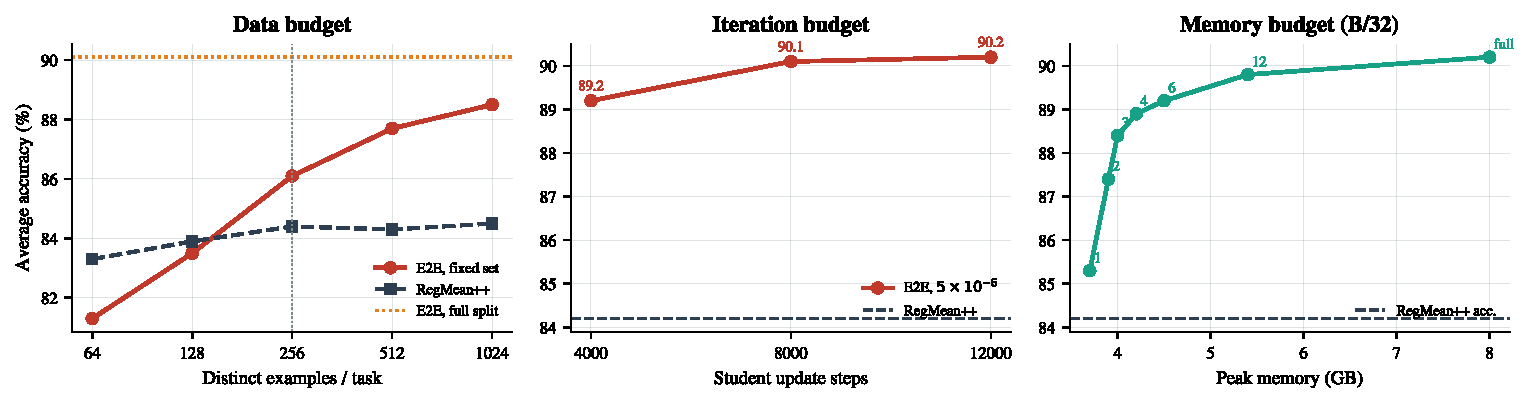
\includegraphics[width=0.98\textwidth]{fig_budget_frontiers.pdf}
\caption{Three measured slices of the accuracy--efficiency frontier, all from existing
ViT-B/32 results.
Left: with a fixed set, RegMean++ leads at $64$--$128$ distinct examples per task, while end-to-end refinement crosses it at $256$; full-split reshuffling reaches $90.1\%$.
Middle: at the selected learning rate, $4$k, $8$k, and $12$k student updates reach $89.2\%$, $90.1\%$, and $90.2\%$ versus RegMean++ at $84.2\%$.
Right: block-wise and canonical full refinement trade peak memory for accuracy; labels denote jointly optimized blocks, and ``full'' is the canonical approximately $8$ GB endpoint.
These are one-dimensional slices, not a jointly compute-matched Pareto surface.}
\label{fig:budget-frontiers}
\end{figure*}

\paragraph{Data frontier.}
At $N=64$ and $128$ distinct examples per task, RegMean++ obtains $83.3\%$ and $83.9\%$, above the fixed-set E2E values $81.3\%$ and $83.5\%$.
At $N=256$, the ordering reverses: $86.1\%$ versus $84.4\%$, and the E2E lead grows to $3.4$ and $4.0$ points at $512$ and $1024$.
This is the cleanest observed regime crossover: an analytic regression estimate is more sample efficient under extreme scarcity, whereas the more expressive objective pays once enough distinct inputs are available.
The methods use the same unique examples at each $N$, but not the same sample exposure or compute.

\paragraph{Iteration frontier.}
For the selected $5\times10^{-6}$ learning rate, the existing $4$k, $8$k, and $12$k measurements yield the sequence in Table~\ref{tab:step-increments}.
\begin{table}[tb]
\centering
\small
\setlength{\tabcolsep}{4pt}
\begin{tabular*}{\columnwidth}{@{\extracolsep{\fill}}lrrr}
\toprule
Point & Updates & Acc. & Gain \\
\midrule
RegMean++ & closed form & 84.2 & 0.0 \\
\method & 4k & 89.2 & $+5.0$ \\
\method & 8k & 90.1 & $+5.9$ \\
\method & 12k & 90.2 & $+6.0$ \\
\bottomrule
\end{tabular*}
\caption{Observed ViT-B/32 accuracy--step slice. Step count is a within-\method compute
proxy, not a wall-clock match to RegMean++; the full 12k run takes about 35 minutes.}
\label{tab:step-increments}
\end{table}
The $4$k point already recovers $5.0/6.0=83.3\%$ of the final measured improvement, and $8$k recovers $5.9/6.0=98.3\%$.
The curve therefore displays the predicted crossing and diminishing returns.
We do not infer unmeasured intermediate wall-clock values or fit the theoretical convergence constants.

\paragraph{Memory frontier.}
On ViT-B/32, block-wise refinement moves from $85.3\%$ at $3.7$ GB to $89.8\%$ at $5.4$ GB, with the canonical full run at $90.2\%$ and about $8$ GB.
On ViT-L/14, a single-block schedule reaches $92.0\%$ at about $13$ GB, four-block groups reach $93.0\%$ at about $15$ GB, and the full block-wise run reaches $94.2\%$ at about $31$ GB.
These points show that memory-constrained users need not choose only between closed form and full-network backpropagation.

\subsection{The crossover moves with consolidation difficulty}
\label{sec:difficulty-frontier}

On ViT-B/32, the \method--RegMean++ gap increases from $2.6$ points at two experts to $3.3$ at four, $4.4$ at six, $6.0$ at eight, and $13.7$ at twenty.
For the same twenty TALL tasks, the margin over the best evaluated baseline is $9.5$ on ViT-L/14, $12.0$ on ViT-B/16, and $13.7$ on ViT-B/32.
These are operational stress axes rather than a proof of a universal scalar interference law, but they agree with the structural-gap account: when a local or restricted compromise is farther from the shared end-to-end function, additional distillation compute buys more.

\begin{figure}[tb]
\centering
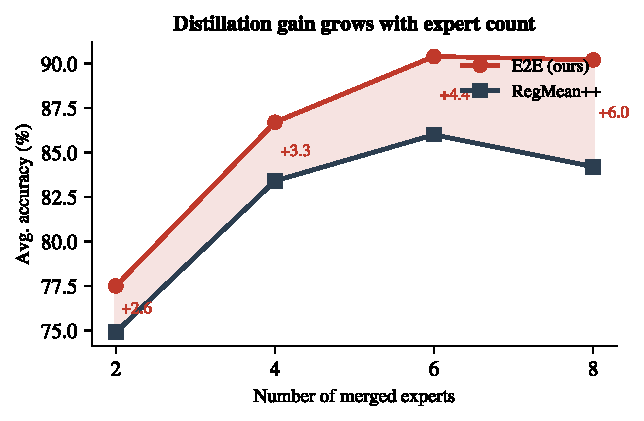
\includegraphics[width=0.94\columnwidth]{fig_scaling.pdf}
\caption{Average ViT-B/32 accuracy as the number of merged experts increases. The
\method--RegMean++ margin grows from $2.6$ to $6.0$ points across the reported two- to eight-expert subsets; the twenty-expert margin is $13.7$ points.}
\label{fig:scaling-main}
\end{figure}

The preliminary Flan-T5 GLUE study supplies the opposite case.
Closed-form RegMean reaches $83.0\%$, while iterative E2E matching reaches $81.9\%$; both beat task arithmetic ($79.0\%$) and TIES ($80.2\%$).
Because RegMean matches layer activations whereas the E2E variant matches the first-step output distribution, this is not a like-for-like solver comparison.
It nevertheless demonstrates that the iterative endpoint is not universally best and motivates the regime view rather than an unconditional ranking.

\subsection{Target choice and the structural mechanism}

\begin{table}[tb]
\centering
\small
\setlength{\tabcolsep}{4pt}
\begin{tabular}{llrr}
\toprule
Backbone & Initialization & Logit KL & Representation \\
\midrule
ViT-B/32 & pre-trained & 87.9 & 89.5 \\
ViT-B/32 & task arithmetic & 88.0 & 90.2 \\
ViT-L/14 & pre-trained & 92.3 & 94.1 \\
ViT-L/14 & task arithmetic & 92.2 & 94.3 \\
\bottomrule
\end{tabular}
\caption{Target-by-initialization control at matched settings within the iterative family.
Representation matching adds $1.6$--$2.2$ points, while the merge initialization adds at most $0.7$ point.}
\label{tab:target-init-main}
\end{table}

The target control supports the head-coverage analysis: representation supervision is the main within-family contributor, not initialization.
The comparison with RegMean++ is broader and simultaneously changes the target scope, update space, trajectory, solver, and compute; it should be read as the overall closed-form-to-end-to-end regime gap, not the isolated effect of gradients.

\begin{figure*}[tb]
\centering
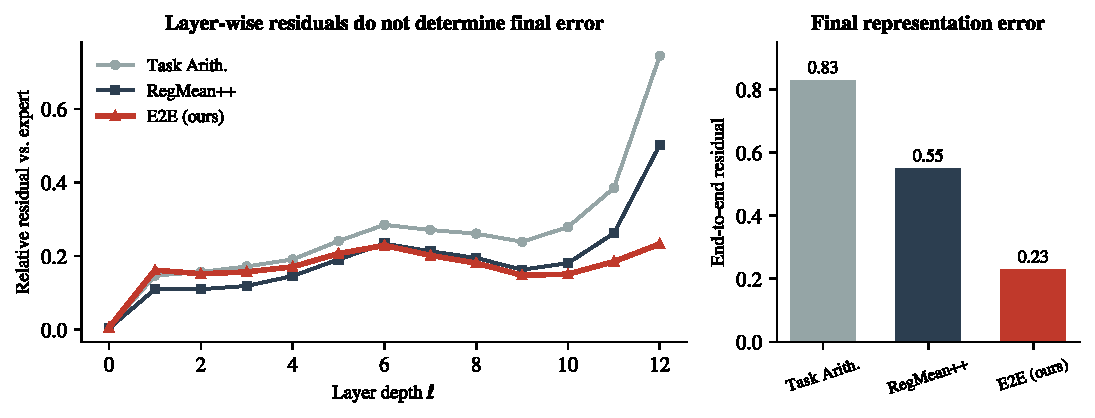
\includegraphics[width=0.82\textwidth]{fig_compound.pdf}
\caption{Layer-wise and final residuals on ViT-B/32. RegMean++ and \method have similar
summed layer-wise residuals ($2.46$ versus $2.11$), but final representation residuals of $0.55$ and $0.23$.
The post-hoc diagnostic uses test inputs only after all model and hyperparameter choices were fixed.}
\label{fig:compound}
\end{figure*}

The residual measurement explains why the higher-compute endpoint can improve: the local regression objective is already small, yet it does not determine the final functional error.
Across task arithmetic, RegMean++, and \method, final residuals $0.83$, $0.55$, and $0.23$ follow the accuracy ordering $67.6$, $84.2$, and $90.2$, whereas the summed layer-wise residual does not.

\subsection{Held-out transfer and statistical stability}
\label{sec:heldout-main}
A budgeted comparison must also check that iterative fitting does not merely trade seen-task accuracy for unseen-task degradation.
Under the two held-out splits used by AdaMerging, the end-to-end model obtains seen/unseen averages of $87.0/66.4$ and $88.4/53.9$.
The strongest closed-form or subspace alternatives reach $81.7/65.8$ and $84.2/53.3$, respectively.
The unseen differences are within seed variation, so the supported conclusion is absence of a measurable seen--unseen penalty rather than a claim of improved zero-shot transfer.

\begin{table}[tb]
\centering
\small
\setlength{\tabcolsep}{3pt}
\begin{tabular*}{\columnwidth}{@{\extracolsep{\fill}}lrrrr}
\toprule
& \multicolumn{2}{c}{Split 1} & \multicolumn{2}{c}{Split 2} \\
Method & Seen & Unseen & Seen & Unseen \\
\midrule
Task Arithmetic & 69.9 & 58.1 & 73.2 & 48.8 \\
Iso-C & 77.0 & 65.8 & 80.2 & 53.3 \\
TSV-M & 81.1 & 65.7 & 83.6 & 51.2 \\
RegMean++ & 81.7 & 63.1 & 84.2 & 52.4 \\
\method & \textbf{87.0} & \textbf{66.4} & \textbf{88.4} & \textbf{53.9} \\
\bottomrule
\end{tabular*}
\caption{Held-out protocol on ViT-B/32: merge six seen experts and evaluate six seen and two unseen tasks. The unseen differences are within seed variation.}
\label{tab:heldout-main}
\end{table}

The available repeated runs give $89.8\pm0.4$ on ViT-B/32, $94.2\pm0.1$ on ViT-L/14, and $92.9\pm0.2$ on TALL-20.
The representative longer ViT-B/32 and ViT-L/14 runs reach $90.2$ and $94.3$; we use the multi-seed means for headline comparisons and retain the longer runs only as measured frontier endpoints.

\paragraph{Deployment contract.}
All operating points return one shared encoder with no learned router or task-specific trainable module, so the additional cost is paid only once before deployment.
CLIP evaluation still selects the fixed class set and text-prototype head associated with each task; ``one model'' therefore refers to the shared encoder rather than a task-agnostic label space.
Inference architecture and encoder cost are unchanged across the compared operating points.

\subsection{Practical choice within the studied settings}

\begin{table}[tb]
\centering
\small
\setlength{\tabcolsep}{4pt}
\begin{tabular}{p{0.63\columnwidth}p{0.29\columnwidth}}
\toprule
Observed evidence & Suggested point \\
\midrule
RegMean++ leads at $N=64,128$ & Closed form \\
E2E crosses at $N=256$ and improves with $N$ & Full E2E \\
Peak-memory budget between the endpoints & Block-wise \\
TALL-20 margins grow to $9.5$--$13.7$ points & Favor E2E \\
GLUE: RegMean $83.0$ vs. E2E $81.9$ (different targets) & Retain closed form \\
\bottomrule
\end{tabular}
\caption{Empirical regime map within the studied settings. It is a decision aid, not a
universal theorem or an exhaustive field-wide comparison.}
\label{tab:regime-map}
\end{table}

\paragraph{A conservative decision procedure.}
Within the measured CLIP setting, start from a closed-form solution when the calibration set is tiny or only statistics-pass compute is available.
At $256$ distinct examples per task, end-to-end refinement becomes more accurate in the ViT-B/32 sweep.
A $4$k-step run captures most of the final measured gain and $8$k is near the observed plateau.
Under activation-memory constraints, block-wise refinement supplies intermediate points.
The larger gains for twenty experts and weaker backbones suggest prioritizing iterative budget where the local compromise is most stressed.
These thresholds are benchmark-specific and should be re-estimated for a new architecture.

\subsection{Reporting efficiency without a fragile scalar score}
\label{sec:efficiency-metrics}
A ratio such as accuracy divided by minutes is not invariant to the accuracy origin, hardware, or resource being constrained.
We instead recommend reporting a resource vector $r=(n,K,M,t)$ containing distinct examples, student updates, peak memory, and measured wall-clock.
Method $i$ Pareto-dominates method $j$ only if it is no worse in accuracy and in every reported resource, and is strictly better in at least one.
Under a single scalar budget $B$, a complementary quantity is the budgeted envelope
\begin{equation}
A^\star(B)=\max_{m:\,C_m\le B} A_m,
\label{eq:budget-envelope-main}
\end{equation}
where $C_m$ must be specified as steps, measured time, memory, or another concrete resource.
For a target expert-relative gap $\epsilon$, one may instead report the cost to target
\begin{equation}
C_m(\epsilon)=\min\{C:\,A_{\mathrm{expert}}-A_m(C)\le\epsilon\}.
\label{eq:cost-target-main}
\end{equation}
The present data support separate slices in $n$, $K$, and $M$, plus three measured endpoint times; they do not support a fully joint Pareto surface or unmeasured wall-clock interpolation.
This distinction is important for using the regime map as evidence rather than as a universal hardware-independent ranking.

\section{Scope and Limitations}
\label{sec:limitations-main}
This is a representative rather than exhaustive comparison.
The clean target control is within the iterative family; RegMean++ versus full E2E also changes trajectory, update freedom, solver, sample exposure, and compute, so it measures an overall regime gap rather than one component.
The main study is CLIP-centric, all experts share a pre-trained initialization, and the Flan-T5 comparison uses different functional readouts.
The break-even results are conditional local bounds, not an AdamW convergence guarantee.
The method is label-free but not data-free: it requires unlabeled inputs, repeated teacher queries, and access to the frozen experts.

\section{Conclusion}
\label{sec:conclusion}

Closed-form merging and end-to-end distillation are best viewed as different budget regimes of functional model consolidation.
Closed-form regression spends little compute and exactly solves a local surrogate, which is advantageous under severe sample or compute constraints and when that surrogate is tight.
Distillation spends teacher queries and student backward passes to reduce the end-to-end functional discrepancy; it becomes worthwhile once its finite-data and optimization errors fall below the closed-form structural gap.
Existing measurements reveal this crossover across data, iteration, memory, expert count, backbone strength, and a preliminary language-model probe.
The result is not a universal winner, but a practical accuracy--efficiency frontier with closed-form, block-wise, and full end-to-end operating points.

\bibliography{references}

\appendix
\section{Algorithmic Details}
\label{app:algorithm}

\subsection{Full procedure}
The student is initialized at the task-arithmetic point $\theta_0+\alpha\sum_a(\theta_a-\theta_0)$.
All experts are frozen.
At each update, we sample one task uniformly, draw a minibatch from that task's finite training split, compute the expert representation without gradients, and update the student with the squared representation loss $\norm{g_\theta(x)-\operatorname{sg}(g_{\theta_a}(x))}_2^2$, where $g$ is the normalized projected CLIP representation and $\operatorname{sg}$ is stop-gradient.
The classification head is never trained.

\subsection{Full-split sampling versus a fixed subset}
The implementation repeatedly reshuffles and cycles each finite training split.
It does not receive infinitely many distinct samples.
Under uniform task and example sampling, the raw minibatch gradient is unbiased for the empirical objective over the finite splits; AdamW and gradient clipping transform that gradient, so the parameter update is not itself an unbiased SGD update.
The fixed-subset comparison in Appendix~\ref{app:sample-budget} is therefore an empirical sample-coverage study, not a population convergence theorem.

\subsection{Cost and memory}
\label{app:cost}
Each update uses one frozen-teacher forward pass and one student forward/backward pass.
The number of teachers affects storage and teacher selection, not the number queried per step.
The measured full-run costs are:

\begin{table}[!ht]
\centering
{\small
\begin{tabular*}{\columnwidth}{@{\extracolsep{\fill}}lrrrr}
\toprule
Setting & Steps & Batch & Minutes & Peak GB \\
\midrule
ViT-B/32, 8 tasks & 12,000 & 32 & $\sim35$ & $\sim8$ \\
ViT-L/14, 8 tasks & 8,000 & 32 & $\sim13$ & $\sim31$ \\
ViT-L/14, 20 tasks & 16,000 & 16 & $\sim34$ & $\sim24$ \\
\bottomrule
\end{tabular*}
}
\caption{Measured one-time offline cost on one RTX 6000 Ada. Intermediate
wall-clock values are not interpolated from these endpoints.}
\label{tab:cost-app}
\end{table}

Closed-form and subspace methods remain substantially cheaper.
RegMean++ requires a statistics pass and linear solves, whereas \method spends thousands of iterative updates.
The selected-rate ViT-B/32 accuracy--step sequence reported in the main paper shows the empirical diminishing-return pattern.
A separate 2,000-step run at learning rate $10^{-5}$ reaches $86.9\%$, above RegMean++; because it uses a different learning rate, it is not included in the clean $5\times10^{-6}$ frontier in the main paper.

\subsection{Optimization-based controls}
\label{app:optimization-controls}
Layer-wise AdaMerging reaches $82.6\%$ on the ViT-B/32 eight-task setting under the same FusionBench harness, below RegMean++ ($84.2\%$) and \method ($90.2\%$).
This indicates that gradient computation alone is insufficient.
The comparison is not a fully factorized estimate of full-weight freedom because AdaMerging also uses an entropy objective.
The target-by-initialization table in the main text is the clean control for the matching target within one optimization family.
\section{Theoretical Analysis}
\label{app:theory}

This appendix proves the results stated in the analysis section of the main paper.
The analysis treats closed-form merging and end-to-end distillation as two computational regimes of the same functional consolidation problem.
It combines an exact local approximation-gap framework with conditional finite-data and compute bounds.
The individual mathematical tools are standard; the contribution is their organization into a budgeted model-consolidation analysis.
The results characterize objectives and local regimes, not global convergence guarantees for AdamW.

\subsection{Formal setup}
Let $A\in\{1,\ldots,T\}$ satisfy $\Pr(A=a)=\pi_a>0$, with $\sum_a\pi_a=1$, and let $X\mid A=a\sim\mathcal D_a$.
Expert $a$ has representation $u_a(x)=g_{\theta_a}(x)\in\mathbb R^d$, and the random teacher target is $Z=u_A(X)$.
Unless stated otherwise, expectations are over this joint task--input distribution.
For a shared measurable map $h$, define
\begin{equation}
    \mathcal F(h)=\mathbb E\|h(X)-Z\|_2^2.
    \label{eq:appendix-F}
\end{equation}
For a parametric merged model, $h=g_\theta$.

\subsection{Bayes target and irreducible teacher conflict}
\label{app:bayes}

\begin{theorem}[Bayes decomposition]
\label{thm:bayes}
Let $\mu(x)=\mathbb E[Z\mid X=x]$.
Then, for every measurable $h$ with finite second moment,
\begin{equation}
\mathcal F(h)=
\mathbb E\|h(X)-\mu(X)\|_2^2
+\mathbb E\|Z-\mu(X)\|_2^2.
\label{eq:bayes-decomposition}
\end{equation}
Consequently, $\mu$ is the Bayes-optimal unconstrained shared function.
If $q_a(x)=\Pr(A=a\mid X=x)$, then the conditional irreducible conflict equals
\begin{equation}
\begin{aligned}
&\sum_a q_a(x)\|u_a(x)-\mu(x)\|_2^2 \\
&\quad=\frac12\sum_{a,b}q_a(x)q_b(x)
\|u_a(x)-u_b(x)\|_2^2.
\end{aligned}
\label{eq:pairwise-conflict}
\end{equation}
\end{theorem}

\begin{proof}
Write $h(X)-Z=(h(X)-\mu(X))+(\mu(X)-Z)$.
Expanding the squared norm, the cross term has expectation
\begin{align*}
&\mathbb E\!\left[
\left\langle h(X)-\mu(X),\mu(X)-Z\right\rangle
\right] \\
&\quad=
\mathbb E\!\left[
\left\langle h(X)-\mu(X),
\mathbb E[\mu(X)-Z\mid X]
\right\rangle
\right]=0.
\end{align*}
This proves Eq.~\eqref{eq:bayes-decomposition}.
For the pairwise identity, condition on $X=x$, abbreviate $q_a=q_a(x)$ and $u_a=u_a(x)$, and use $\mu=\sum_aq_au_a$:
\begin{align*}
\frac12\sum_{a,b}q_aq_b\|u_a-u_b\|_2^2
&=\sum_aq_a\|u_a\|_2^2-
\left\|\sum_aq_au_a\right\|_2^2 \\
&=\sum_aq_a\|u_a-\mu\|_2^2.
\end{align*}
\end{proof}

Equation~\eqref{eq:bayes-decomposition} distinguishes two obstacles.
The second term is conflict among teacher functions on overlapping input support and cannot be removed by any shared predictor.
The first term is approximation error within the shared model class.
If the task is identifiable from the input, $q_a(x)$ is concentrated and the Bayes target reduces to the corresponding expert.
If several tasks assign different expert representations to the same input, the Bayes target is their posterior-weighted average rather than any one teacher.

\subsection{From representation residual to accuracy}
\label{app:accuracy}

For task $a$, let $\mathcal C_a$ be its class set and let the fixed head score class $c$ by $s_{a,c}(u)=\langle t_{a,c},u\rangle$, with $\|t_{a,c}\|_2\le1$.
A common positive CLIP logit scale does not change the argmax.
Let $c_a^*(x)$ be expert $a$'s predicted class and define the expert top-two margin
\begin{equation}
\gamma_a(x)=s_{a,c_a^*(x)}(u_a(x))-
\max_{c\ne c_a^*(x)}s_{a,c}(u_a(x)).
\label{eq:expert-margin}
\end{equation}

\begin{proposition}[Pointwise prediction preservation]
\label{prop:pointwise-margin}
If $\|g_\theta(x)-u_a(x)\|_2<\gamma_a(x)/2$, then the merged model and expert $a$ predict the same class on $x$.
\end{proposition}

\begin{proof}
Let $\delta=g_\theta(x)-u_a(x)$.
For every class $c$, $|\langle t_{a,c},\delta\rangle|\le\|\delta\|_2$.
Hence the gap between the expert's top class and any competitor decreases by at most $2\|\delta\|_2$.
The assumed inequality keeps every gap positive.
\end{proof}

\begin{corollary}[Expected representation loss bounds the accuracy gap]
\label{cor:accuracy-gap}
Define $F_a(\theta)=\mathbb E_{X\sim\mathcal D_a} \|g_\theta(X)-u_a(X)\|_2^2$.
For every $\gamma_0>0$,
\begin{equation}
\left|\operatorname{Acc}_a(\theta)-\operatorname{Acc}_a(\theta_a)\right|
\le
\Pr[\gamma_a(X)\le\gamma_0]
+\frac{4F_a(\theta)}{\gamma_0^2}.
\label{eq:accuracy-gap}
\end{equation}
\end{corollary}

\begin{proof}
The absolute difference of the two correctness indicators is at most the indicator that the two predictors disagree.
By Proposition~\ref{prop:pointwise-margin}, disagreement is contained in the event $2\|g_\theta(X)-u_a(X)\|_2\ge\gamma_a(X)$.
Split this event according to whether $\gamma_a(X)\le\gamma_0$, then apply Markov's inequality to the squared residual on the complementary event.
\end{proof}

The bound is relative to the expert, not directly to Bayes-optimal ground-truth risk.
It is nevertheless the relevant guarantee for a merger whose stated goal is to preserve the expert functions.

\subsection{Head-frame characterization of logit supervision}
\label{app:head-frame}

Let $T_a=[t_{a,1},\ldots,t_{a,C_a}]\in\mathbb R^{d\times C_a}$.
For a representation error $v$, squared-logit discrepancy is $\|T_a^\top v\|_2^2=v^\top T_aT_a^\top v$.

\begin{theorem}[Frame bounds and exact equivalence]
\label{thm:frame}
For nonnegative weights $\omega_a$, define $S=\sum_a\omega_aT_aT_a^\top$.
Then, for every $v\in\mathbb R^d$,
\begin{equation}
\lambda_{\min}(S)\|v\|_2^2
\le\sum_a\omega_a\|T_a^\top v\|_2^2
\le\lambda_{\max}(S)\|v\|_2^2.
\label{eq:frame-bounds}
\end{equation}
The aggregate logit seminorm is norm-equivalent to the representation norm on $\mathbb R^d$ if and only if $S\succ0$.
If $S$ is singular, there exists a nonzero $v$ with zero discrepancy under every included head for which $\omega_a>0$.
\end{theorem}

\begin{proof}
The middle quantity equals $v^\top Sv$.
The inequalities are the Rayleigh quotient bounds.
It is a norm exactly when its null space is trivial, equivalently when $S\succ0$.
If $S$ is singular, choose any nonzero $v\in\ker S$.
Since all summands are nonnegative, $0=v^\top Sv=\sum_a\omega_a\|T_a^\top v\|_2^2$ implies $T_a^\top v=0$ for every positively weighted head.
\end{proof}

The condition number $\lambda_{\max}(S)/\lambda_{\min}(S)$ quantifies how unevenly the heads supervise different directions when $S\succ0$.
In the actual task-conditioned loss, task $a$ applies only $T_a$ to its own error, so the relevant per-task operator is $T_aT_a^\top$ rather than the union operator $S$.

\begin{proposition}[Local geometry of KL distillation]
\label{prop:kl-geometry}
Let $p_a=\operatorname{softmax}(\beta_aT_a^\top u_a)$, where $u_a$ is the teacher representation and $\beta_a>0$ is the CLIP logit scale (softmax temperature), and perturb the representation by $v$.
In a neighborhood of $v=0$,
\begin{align}
&D_{\mathrm{KL}}\!\left(
 p_a\,\middle\|\,
 \operatorname{softmax}(\beta_aT_a^\top(u_a+v))
 \right) \\
&\qquad=
\frac12 v^\top G_a v
+O\!\left(\|\beta_aT_a^\top v\|_2^3\right),
\label{eq:kl-expansion}
\end{align}
where
\begin{equation}
G_a=\beta_a^2T_a
\left(\operatorname{Diag}(p_a)-p_ap_a^\top\right)T_a^\top\succeq0.
\label{eq:kl-metric}
\end{equation}
Its range is contained in $\operatorname{span}(T_a)$.
\end{proposition}

\begin{proof}
As a function of logits $z$, the cross-entropy with fixed target $p_a$ has Hessian $\operatorname{Diag}(p_a)-p_ap_a^\top$ at the teacher logits, and its gradient vanishes there.
Taylor expansion with logit perturbation $\beta_aT_a^\top v$ gives the result.
The range statement follows from the left and right multiplication by $T_a$ and $T_a^\top$.
\end{proof}

Representation matching uses the identity metric and therefore controls every linear head by $\|\widetilde T^\top v\|_2\le\|\widetilde T\|_{\mathrm{op}}\|v\|_2$, where $\widetilde T=[\,T_1,\dots,T_T\,]$ concatenates the per-task prototype matrices of all $T$ tasks column-wise.
The theorem and proposition identify a structural information difference; empirical superiority remains a question for the controlled target comparison.

\subsection{Local functional geometry and exact surrogate gap}
\label{app:local-gap}

Fix a reference merge $\bar\theta$ and define the residual $r_a(x)=g_{\bar\theta}(x)-g_{\theta_a}(x)$ and Jacobian $J(x)=\nabla_\theta g_{\bar\theta}(x)$.
The first-order residual model is $r_a(x)+J(x)\Delta$.
With damping $\lambda>0$, define
\begin{align}
Q(\Delta)
&=\frac12\mathbb E\|r_A(X)+J(X)\Delta\|_2^2
  +\frac\lambda2\|\Delta\|_2^2 \\
&=C-b^\top\Delta+\frac12\Delta^\top H\Delta,
\label{eq:Q-def}
\end{align}
where
\begin{equation}
H=\mathbb E[J^\top J]+\lambda I\succ0,
\qquad
b=-\mathbb E[J^\top r_A(X)].
\label{eq:H-b}
\end{equation}
The unique optimum is $\Delta^\star=H^{-1}b$.

\begin{theorem}[Exact local excess loss]
\label{thm:exact-gap}
For every update $\widetilde\Delta$,
\begin{equation}
Q(\widetilde\Delta)-Q(\Delta^\star)
=\frac12\|\widetilde\Delta-\Delta^\star\|_H^2
=\frac12\|H\widetilde\Delta-b\|_{H^{-1}}^2.
\label{eq:exact-gap}
\end{equation}
If $\widetilde\Delta$ solves $\widetilde H\widetilde\Delta=\widetilde b$, then
\begin{equation}
H\widetilde\Delta-b
=(H-\widetilde H)\widetilde\Delta+(\widetilde b-b).
\label{eq:surrogate-residual}
\end{equation}
\end{theorem}

\begin{proof}
Using $b=H\Delta^\star$ and completing the square gives $Q(\Delta)=Q(\Delta^\star)+ \frac12(\Delta-\Delta^\star)^\top H(\Delta-\Delta^\star)$.
Also, $H\widetilde\Delta-b=H(\widetilde\Delta-\Delta^\star)$, which proves the second equality.
Substituting $\widetilde H\widetilde\Delta=\widetilde b$ gives Eq.~\eqref{eq:surrogate-residual}.
\end{proof}

The two terms in Eq.~\eqref{eq:surrogate-residual} need not contribute additively because the $H^{-1}$ norm includes a cross term.
The exact statement is that geometry mismatch and target/trajectory mismatch jointly determine the normal-equation residual.
This is stronger and more precise than merely observing that the full feasible set contains a surrogate solution.

\subsection{Exact cost of a restricted update subspace}
\label{app:subspace-gap}

\begin{theorem}[Functional projection gap]
\label{thm:subspace-gap}
Let $U\in\mathbb R^{p\times k}$ have full column rank and restrict $\Delta=Uc$ for a coefficient vector $c$.
The best restricted update is
\begin{equation}
\Delta_U
=U(U^\top HU)^{-1}U^\top b.
\label{eq:restricted-update}
\end{equation}
Let $P_U^H=U(U^\top HU)^{-1}U^\top H$ be the $H$-orthogonal projection onto $\operatorname{col}(U)$.
Then
\begin{equation}
Q(\Delta_U)-Q(\Delta^\star)
=\frac12\|(I-P_U^H)\Delta^\star\|_H^2.
\label{eq:subspace-gap}
\end{equation}
\end{theorem}

\begin{proof}
Differentiating $Q(Uc)$ gives $U^\top HUc=U^\top b$, which yields Eq.~\eqref{eq:restricted-update}.
Since $b=H\Delta^\star$, $\Delta_U=P_U^H\Delta^\star$.
Apply Theorem~\ref{thm:exact-gap}.
\end{proof}

Equation~\eqref{eq:subspace-gap} isolates update freedom while holding the local functional target and metric fixed.
Actual coefficient methods may additionally optimize entropy or another target, in which case Theorem~\ref{thm:exact-gap} contributes an additional surrogate mismatch.

\subsection{Exact cost of dropping cross-layer coupling}
\label{app:cross-layer-gap}

Partition parameters by layer or block and write $H=D+E$, where $D=\operatorname{blockdiag}(H_{11},\ldots,H_{LL})$ and $E$ contains the off-diagonal blocks.
Assume $D\succ0$ and define the independent block solution $\Delta_D=D^{-1}b$.

\begin{theorem}[Cross-layer coupling gap]
\label{thm:cross-layer-gap}
The excess local objective of the block-diagonal solve is
\begin{equation}
Q(\Delta_D)-Q(\Delta^\star)
=\frac12\|E\Delta_D\|_{H^{-1}}^2.
\label{eq:cross-layer-gap}
\end{equation}
If $\lambda_{\min}I\preceq H\preceq\lambda_{\max}I$, then
\begin{equation}
\frac{1}{2\lambda_{\max}}\|E\Delta_D\|_2^2
\le Q(\Delta_D)-Q(\Delta^\star)
\le\frac{1}{2\lambda_{\min}}\|E\Delta_D\|_2^2.
\label{eq:cross-layer-bounds}
\end{equation}
The independent solve is exact if and only if $E\Delta_D=0$.
\end{theorem}

\begin{proof}
Because $D\Delta_D=b$, $H\Delta_D-b=(D+E)\Delta_D-b=E\Delta_D$.
Apply Theorem~\ref{thm:exact-gap}.
The spectral bounds follow from $\lambda_{\max}^{-1}I\preceq H^{-1}\preceq\lambda_{\min}^{-1}I$.
\end{proof}

The gap can be arbitrarily large even when every diagonal block is perfectly conditioned.
Let \[ H_\rho=\begin{bmatrix}1&\rho\\ \rho&1\end{bmatrix}, \qquad b=\begin{bmatrix}1\\-1\end{bmatrix}, \qquad 0<\rho<1.
\] Then $D=I$ and $\Delta_D=b$, while $\Delta^\star=(1-\rho)^{-1}b$.
Direct substitution gives
\begin{equation}
Q(\Delta_D)-Q(\Delta^\star)=\frac{\rho^2}{1-\rho},
\label{eq:cross-layer-example}
\end{equation}
which diverges as $\rho\to1$.
The example formalizes why small independent block residuals need not imply a small final functional gap.

\subsection{RegMean as an expert-centered isotropic surrogate}
\label{app:regmean-proof}

Fix a linear layer $\ell$.
Let $h_{a,\ell-1}(x)$ be expert $a$'s input activation, $W_{a,\ell}$ its weight, and $\Phi_{a,\ell}$ the expert suffix from that layer's output to the final representation.
Define $z_{a,\ell}(x)=W_{a,\ell}h_{a,\ell-1}(x)$ and the suffix Jacobian \[ D_{a,\ell}(x)= \left.\frac{\partial\Phi_{a,\ell}(z)}{\partial z} \right|_{z=z_{a,\ell}(x)}.
\] The expert-trajectory, first-order one-layer surrogate is
\begin{equation}
\widetilde F_\ell(W)=
\frac12\sum_a\pi_a\mathbb E
\left\|
D_{a,\ell}(X)(W-W_{a,\ell})h_{a,\ell-1}(X)
\right\|_2^2.
\label{eq:regmean-surrogate}
\end{equation}
This is a separately defined local surrogate.
It is not the original nonlinear objective with all but one layer frozen, because both terms are evaluated on the expert activation and through the expert suffix.

\begin{assumption}[Shared isotropic downstream metric]
\label{ass:isotropic}
On the residual directions appearing in Eq.~\eqref{eq:regmean-surrogate}, $D_{a,\ell}(x)^\top D_{a,\ell}(x)=c_\ell I$ for a constant $c_\ell>0$ shared across experts and samples.
\end{assumption}

\begin{proposition}[RegMean solution]
\label{prop:regmean-formal}
Let $G_{a,\ell}=\mathbb E[h_{a,\ell-1}(X)h_{a,\ell-1}(X)^\top]$.
Under Assumption~\ref{ass:isotropic}, minimizing Eq.~\eqref{eq:regmean-surrogate} is equivalent to RegMean's layer regression.
If $\sum_a\pi_aG_{a,\ell}\succ0$, the unique minimizer is
\begin{equation}
W_{\mathrm{RM},\ell}
=\left(\sum_a\pi_aW_{a,\ell}G_{a,\ell}\right)
 \left(\sum_a\pi_aG_{a,\ell}\right)^{-1}.
\label{eq:regmean-solution}
\end{equation}
\end{proposition}

\begin{proof}
Assumption~\ref{ass:isotropic} converts each term of Eq.~\eqref{eq:regmean-surrogate} into $c_\ell\|(W-W_{a,\ell})h_{a,\ell-1}(X)\|_2^2/2$.
Differentiation gives $\sum_a\pi_a(W-W_{a,\ell})G_{a,\ell}=0$, whose unique solution is Eq.~\eqref{eq:regmean-solution}.
\end{proof}

Relative to the full functional objective, this construction makes four approximations: (1) one layer is changed at a time; (2) expert rather than current merged activations are used; (3) the downstream map is linearized on the expert trajectory; and (4) its metric is replaced by a shared isotropic one.
RegMean++ reduces the activation mismatch by propagating the partially merged model, but remains layer-local and does not retain the full downstream metric or all off-diagonal blocks of $H$.

\subsection{Parameter-space metric surrogates}
\label{app:parameter-metrics}

A broad parameter-space family minimizes
\begin{equation}
\mathcal Q_M(\theta)=
\sum_a\pi_a(\theta-\theta_a)^\top M_a(\theta-\theta_a),
\qquad M_a\succeq0.
\label{eq:parameter-metric}
\end{equation}
If $M=\sum_a\pi_aM_a\succ0$, its solution is
\begin{equation}
\theta_M=M^{-1}\sum_a\pi_aM_a\theta_a.
\label{eq:parameter-metric-solution}
\end{equation}
Uniform averaging uses $M_a=I$; Fisher merging uses a diagonal classification-Fisher approximation.
If the network were linear in parameters, $g_\theta(x)=\Phi(x)\theta$, then the exact local functional metric would be $M_a=\mathbb E[\Phi(X)^\top\Phi(X)]$.
In a nonlinear network, a fixed identity or diagonal metric is generally a surrogate for the input-dependent functional pullback $\mathbb E[J^\top J]$.

\subsection{Nonlinear remainder of a fixed residual model}
\label{app:nonlinear}

The previous gap formulas are exact for the damped linearized objective $Q$.
We now bound the mismatch between that objective and the nonlinear representation loss.

\begin{proposition}[Residual-linearization remainder]
\label{prop:nonlinear-remainder}
For each task--input pair, let $r(\theta)=g_\theta(x)-g_{\theta_a}(x)$.
Suppose on the segment from $\bar\theta$ to $\bar\theta+\Delta$ that the Jacobian is $L_J$-Lipschitz, $\|r(\bar\theta)\|_2\le R$, and $\|J(\bar\theta)\|_{\mathrm{op}}\le B$.
Let $q(\Delta)=\frac12\|r(\bar\theta)+J(\bar\theta)\Delta\|_2^2$.
Then
\begin{align}
&\left|
\frac12\|r(\bar\theta+\Delta)\|_2^2-q(\Delta)
\right| \\
&\quad\le
\frac{L_J}{2}(R+B\|\Delta\|_2)\|\Delta\|_2^2
+\frac{L_J^2}{8}\|\Delta\|_2^4.
\label{eq:nonlinear-remainder}
\end{align}
The same bound holds after expectation when the constants are uniform.
\end{proposition}

\begin{proof}
Taylor's theorem for the vector residual gives $r(\bar\theta+\Delta)=r(\bar\theta)+J(\bar\theta)\Delta+e$ with $\|e\|_2\le L_J\|\Delta\|_2^2/2$.
Expanding the squared norm yields the difference $\langle r+J\Delta,e\rangle+\|e\|_2^2/2$.
Apply Cauchy--Schwarz and the stated bounds.
\end{proof}

A one-shot regression or quadratic solve is accurate only while this remainder and the surrogate mismatches are small.
End-to-end optimization repeatedly updates the true nonlinear residual and thereby relinearizes along the current merged trajectory.
The proposition does not guarantee a better global optimum or a convergence rate.

\subsection{Compute-dependent refinement and break-even}
\label{app:compute-error}

We now formalize the additional issue that closed-form and end-to-end methods occupy different compute regimes.
Let $F(\theta)=\mathcal F(g_\theta)$, $F^\star=\inf_{\theta\in\Theta}F(\theta)$, and define
\begin{equation}
\Delta_{\mathrm{RM}}=F(\theta_{\mathrm{RM}})-F^\star,
\qquad
\Delta_k=F(\theta_k)-F^\star.
\label{eq:formal-gaps}
\end{equation}
RegMean analytically solves the finite-sample layer-wise surrogate in Eq.~\eqref{eq:regmean-surrogate}; the remaining $\Delta_{\mathrm{RM}}$ is its gap on the full nonlinear objective and need not vanish.
The same fixed-gap interpretation applies to a sequential closed-form variant such as RegMean++ once its output is fixed; the experiments use RegMean++ as the stronger reference.
End-to-end refinement instead produces a sequence $\Delta_k$ whose decrease requires iterative computation.

\begin{proposition}[Idealized descent and local linear rate]
\label{prop:compute-error-formal}
Suppose $F$ is differentiable and $L$-smooth on a region containing the full-gradient iterates
\begin{equation}
\theta_{k+1}=\theta_k-\eta\nabla F(\theta_k),
\qquad 0<\eta\le 1/L.
\label{eq:idealized-gd}
\end{equation}
Then for every $K\ge1$,
\begin{equation}
F(\theta_K)
\le
F(\theta_0)-\frac{\eta}{2}
\sum_{k=0}^{K-1}\|\nabla F(\theta_k)\|_2^2.
\label{eq:formal-descent}
\end{equation}
If, throughout the same region, $F$ satisfies the Polyak--Lojasiewicz condition
\begin{equation}
\frac12\|\nabla F(\theta)\|_2^2
\ge \mu\bigl(F(\theta)-F^\star\bigr)
\label{eq:pl-condition}
\end{equation}
for some $\mu>0$, then
\begin{equation}
\Delta_K\le(1-\mu\eta)^K\Delta_0.
\label{eq:formal-linear-rate}
\end{equation}
\end{proposition}

\begin{proof}
$L$-smoothness gives
\begin{align*}
F(\theta_{k+1})
&\le F(\theta_k)
+\langle\nabla F(\theta_k),
  \theta_{k+1}-\theta_k\rangle \\
&\quad +\frac L2
  \|\theta_{k+1}-\theta_k\|_2^2 \\
&=F(\theta_k)-\eta\left(1-\frac{L\eta}{2}\right)
  \|\nabla F(\theta_k)\|_2^2 \\
&\le F(\theta_k)-\frac\eta2
  \|\nabla F(\theta_k)\|_2^2.
\end{align*}
Summing proves Eq.~\eqref{eq:formal-descent}.
Under Eq.~\eqref{eq:pl-condition}, the one-step inequality becomes $\Delta_{k+1}\le(1-\mu\eta)\Delta_k$; induction gives Eq.~\eqref{eq:formal-linear-rate}.
\end{proof}

\begin{corollary}[Break-even refinement budget]
\label{cor:break-even-formal}
Assume the conditions of Proposition~\ref{prop:compute-error-formal}, $0<\mu\eta<1$, and $0<\Delta_{\mathrm{RM}}<\Delta_0$.
Define
\begin{equation}
K_{\mathrm{be}}
=
\left\lceil
\frac{\log(\Delta_{\mathrm{RM}}/\Delta_0)}
     {\log(1-\mu\eta)}
\right\rceil.
\label{eq:formal-break-even}
\end{equation}
Then every $K\ge K_{\mathrm{be}}$ satisfies $F(\theta_K)-F^\star\le\Delta_{\mathrm{RM}}$, and hence $F(\theta_K)\le F(\theta_{\mathrm{RM}})$.
\end{corollary}

\begin{proof}
Equation~\eqref{eq:formal-linear-rate} and the definition of $K_{\mathrm{be}}$ imply $(1-\mu\eta)^K\Delta_0\le\Delta_{\mathrm{RM}}$.
\end{proof}

The formula has two boundary cases.
If $\Delta_0\le\Delta_{\mathrm{RM}}$, the initialization is already no worse on $F$; if $\Delta_{\mathrm{RM}}=0$, the closed-form output already attains the best functional value and no method can improve it on this objective.

Let one end-to-end update cost $c_{\mathrm{step}}$ and let $C_K=C_{\mathrm{init}}+Kc_{\mathrm{step}}$.
Since $(1-\mu\eta)^K\le e^{-\mu\eta K}$,
\begin{equation}
\Delta_K
\le
\exp\!\left[-\frac{\mu\eta}{c_{\mathrm{step}}}
(C_K-C_{\mathrm{init}})\right]\Delta_0.
\label{eq:formal-cost-envelope}
\end{equation}
The cost of one practical step consists of one frozen-teacher forward and one student forward--backward pass.
Equation~\eqref{eq:formal-cost-envelope} is therefore a local functional-error envelope as compute increases, not a claim that wall-clock efficiency is identical across hardware or implementations.

The functional envelope also induces an expert-relative accuracy envelope.
Under uniform task weights define
\begin{align}
\overline G(\theta)
&=\frac1T\sum_{a=1}^T
\left|\operatorname{Acc}_a(\theta)-\operatorname{Acc}_a(\theta_a)\right|,\\
m(\gamma_0)
&=\frac1T\sum_{a=1}^T\Pr[\gamma_a(X)\le\gamma_0].
\end{align}
Averaging Corollary~\ref{cor:accuracy-gap} over tasks and applying Eq.~\eqref{eq:formal-linear-rate} gives
\begin{equation}
\overline G(\theta_K)
\le
m(\gamma_0)
+\frac{4}{\gamma_0^2}
\left[F^\star+(1-\mu\eta)^K\Delta_0\right].
\label{eq:accuracy-compute-envelope}
\end{equation}
Thus iterative compute can tighten the optimizable part of the accuracy-gap upper bound, but the envelope plateaus at the Bayes/model-class functional floor and the experts' low-margin mass.

\begin{remark}[Scope of the compute result]
The implemented optimizer is AdamW with clipping and a finite reshuffled training split, not the idealized full-gradient method of Proposition~\ref{prop:compute-error-formal}.
We do not estimate $L$, $\mu$, $F^\star$, or the per-step functional losses needed to fit Eq.~\eqref{eq:formal-linear-rate}.
The reported step sweep is used only to test the qualitative crossing-and-saturation prediction.
Its observed accuracy values are not substituted into the theorem as estimates of $F$.
\end{remark}


\subsection{Finite-data optimization and a sufficient regime condition}
\label{app:finite-data-regime}

The local compute result controls optimization error, while the calibration sweep varies sample coverage.
The following standard uniform-deviation statement makes the two axes explicit without assuming a particular rate for neural networks.

\begin{proposition}[Finite-data functional bound]
\label{prop:finite-data-regime}
Let $\widehat F_n$ be an empirical functional objective and let $F^\star=\inf_{\theta\in\mathcal R}F(\theta)$ on a region $\mathcal R$.
Suppose
\begin{equation}
\sup_{\theta\in\mathcal R}|F(\theta)-\widehat F_n(\theta)|\le\varepsilon_n.
\label{eq:uniform-deviation}
\end{equation}
Let $\widehat\theta_n^\star\in\arg\min_{\theta\in\mathcal R}\widehat F_n(\theta)$ and suppose an iterate $\theta_K\in\mathcal R$ has empirical optimization error
\begin{equation}
\delta_K=
\widehat F_n(\theta_K)-\widehat F_n(\widehat\theta_n^\star)\ge0.
\label{eq:empirical-opt-error}
\end{equation}
Then
\begin{equation}
F(\theta_K)-F^\star\le 2\varepsilon_n+\delta_K.
\label{eq:finite-data-regime-bound}
\end{equation}
Consequently, for any fixed closed-form reference $\theta_{\mathrm{CF}}$ with $\Delta_{\mathrm{CF}}=F(\theta_{\mathrm{CF}})-F^\star$, the sufficient condition
\begin{equation}
2\varepsilon_n+\delta_K<\Delta_{\mathrm{CF}}
\label{eq:sufficient-regime-condition}
\end{equation}
implies $F(\theta_K)<F(\theta_{\mathrm{CF}})$.
\end{proposition}

\begin{proof}
By Eq.~\eqref{eq:uniform-deviation},
\begin{align*}
F(\theta_K)
&\le \widehat F_n(\theta_K)+\varepsilon_n \\
&=\widehat F_n(\widehat\theta_n^\star)+\delta_K+\varepsilon_n \\
&\le \widehat F_n(\theta^\star)+\delta_K+\varepsilon_n \\
&\le F(\theta^\star)+2\varepsilon_n+\delta_K,
\end{align*}
where $\theta^\star\in\arg\min_{\theta\in\mathcal R}F(\theta)$.
This proves Eq.~\eqref{eq:finite-data-regime-bound}; subtracting the closed-form gap gives the final claim.
\end{proof}

The proposition is deliberately conditional.
We do not claim a distribution-free value or rate for $\varepsilon_n$, nor do we estimate it from accuracy.
It formalizes the regime logic tested by the sample sweep: increasing the number of distinct inputs can reduce the finite-data term, while more updates reduce the empirical optimization term.
The closed-form reference may itself depend on finite data; in $\Delta_{\mathrm{CF}}$ that realized estimation effect is already included.
A fully factorized comparison would require separate population surrogates and stability bounds for each merger, which are outside the present evidence.

\subsection{Finite empirical objective}
\label{app:finite-data}

Let $S_a=\{x_{a,1},\ldots,x_{a,n_a}\}$ be the finite training split and define \[ \widehat{\mathcal F}(\theta) =\sum_a\pi_a\frac1{n_a}\sum_{i=1}^{n_a} \|g_\theta(x_{a,i})-g_{\theta_a}(x_{a,i})\|_2^2.
\] Uniformly sampling a task and then an example from its finite split makes the \emph{raw} single-example gradient unbiased for $\nabla\widehat{\mathcal F}$.
Repeated reshuffling does not create new unique samples, and clipping plus AdamW means the update itself is not unbiased SGD.
We therefore make no population-convergence or distribution-free generalization claim from the sampling procedure.

\subsection{Summary of approximation sources}
\label{app:theory-summary}

The theory separates three independent sources of error:
\begin{enumerate}
    \item \textbf{Target information:} a logit or local-KL loss uses a task-head
semimetric; representation matching uses the full shared-space metric.
    \item \textbf{Update freedom:} a coefficient or task-vector family loses the
$H$-energy of the optimal functional update outside its subspace.
    \item \textbf{Local geometry and trajectory:} layer-wise and parameter-metric
surrogates change the normal equations, delete cross-layer blocks, or linearize at a different trajectory; fixed local models also incur the nonlinear remainder.
    \item \textbf{Data and iterative computation:} RegMean removes optimization error only
for its chosen surrogate.
End-to-end refinement pays a finite-data term and an iterative optimization term; increasing distinct sample coverage and update budget can reduce these terms until they fall below the realized closed-form structural gap.
\end{enumerate}
These dimensions need not form a single total ordering.
The experiments test their predicted signatures rather than claim to estimate every matrix term directly.
\section{Experimental Setup and Reproducibility}
\label{app:setup}

\subsection{Evaluation protocol}
All vision experiments use FusionBench \citep{tang2024fusionbench}.
Data-dependent calibration uses only the training split.
Test labels and inputs are not used for optimization, hyperparameter selection, or model selection.
The layer-wise residual diagnostic reported in the main paper uses test inputs only for a post-hoc measurement after every model and hyperparameter was fixed; no test labels enter the diagnostic.

For CLIP, evaluation selects the fixed class set and text-prototype head corresponding to the task.
The merged object is one shared encoder with no learned router, adapter, or per-task trainable module; this should not be read as a task-identity-free classification pipeline.

\subsection{Datasets}
Table~\ref{tab:datasets} lists the twenty classification datasets used throughout, with their domains and class counts.
The eight tasks of the standard benchmark deliberately span dissimilar domains (scenes, fine-grained objects, remote sensing, digits, traffic signs, textures), and the twenty-task extension adds further characters, medical, and rendered-text domains; this domain spread is what makes consolidation nontrivial and is exercised directly by the scaling experiments.

\begin{table*}[tb]
\centering
{\small
\begin{tabular*}{\textwidth}{@{\extracolsep{\fill}}llrllr}
\toprule
Dataset & Domain & Classes & Dataset & Domain & Classes \\
\midrule
SUN397 & scenes & 397 & Flowers102 & flowers & 102 \\
Stanford Cars & fine-grained & 196 & PCAM & histopathology & 2 \\
RESISC45 & remote sensing & 45 & FER2013 & facial emotion & 7 \\
EuroSAT & remote sensing & 10 & Oxford Pets & fine-grained & 37 \\
SVHN & digits & 10 & STL10 & objects & 10 \\
GTSRB & traffic signs & 43 & CIFAR100 & objects & 100 \\
MNIST & digits & 10 & CIFAR10 & objects & 10 \\
DTD & textures & 47 & Food101 & food & 101 \\
FashionMNIST & clothing & 10 & EMNIST letters & characters & 26 \\
KMNIST & characters & 10 & Rendered-SST2 & rendered text & 2 \\
\bottomrule
\end{tabular*}
}
\caption{Datasets. The left eight entries in the first four rows form the standard
TA-8 benchmark; all twenty entries form TALL-20.
We use FusionBench's standard splits and released experts.}
\label{tab:datasets}
\end{table*}

The eight-task benchmark follows task arithmetic \citep{ilharco2023taskarithmetic}; the twenty-task extension follows TALL \citep{wang2024tall}.
The public experts use the corresponding CLIP ViT-B/32, ViT-B/16, or ViT-L/14 backbone.

\subsection{Baselines}
Task Arithmetic uses the FusionBench scale $0.3$.
Fisher uses a diagonal Fisher estimate.
TSV-M and Iso-C use their task-vector subspace formulations.
RegMean++ uses sequential regression with activations from the partially merged model.
TIES and DARE were also run but are below the stronger data-driven baselines in the principal settings.
AdaMerging is reported as an optimization-based coefficient control.

SAMerging has a released implementation \citep{samerging2025}; we did not integrate that code into the present harness.
The reported ``logit+SAM'' row instead applies SAM to our matched KL control and should not be interpreted as an official reproduction.
FeatCal and Output-Space Projection are discussed as closely related methods \citep{featcal2026,outputprojection2026} but are not directly benchmarked in the supplied experiments.
These omissions are stated explicitly rather than hidden behind a state-of-the-art claim.

\subsection{Hyperparameters}
Table~\ref{tab:hyperparameters} collects the default \method configuration used unless a specific experiment states otherwise.
A single setting transfers across all three backbones and both benchmark sizes---only the batch size and step budget change for the larger TALL-20 pool---so the gains reported elsewhere do not rely on per-setting tuning.

\begin{table}[tb]
\centering
{\small
\begin{tabular}{p{0.92in}p{0.72in}p{1.18in}}
\toprule
Hyperparameter & Value & Note \\
\midrule
Init. scale $\alpha$ & $0.3$ & task-arithmetic start \\
Optimizer & AdamW & $\beta=(0.9,0.999)$; no weight decay \\
Learning rate & $5\times10^{-6}$ & selected from sweep \\
Gradient clip & $1.0$ & global norm \\
Batch size & $32$ & $16$ for TALL-20 \\
Steps & $8$--$12$k & $16$k for TALL-20 \\
Target & norm. projection & squared distance \\
\bottomrule
\end{tabular}
}
\caption{Default \method hyperparameters. Detailed step counts are stated with each
result; no labels are used.}
\label{tab:hyperparameters}
\end{table}

The main multi-seed eight-task runs use 8,000 steps.
The longer representative ViT-B/32 and ViT-L/14 rows in the per-task tables use 12,000 steps.
The TALL-20 runs use 16,000 steps.
This distinction prevents a representative longer run from being mistaken for a multi-seed mean.

\subsection{Reproduction interface}
The implementation is a FusionBench method with a fixed configuration.
A representative command has the form
\begin{quote}\footnotesize\ttfamily\raggedright
fusion\_bench method=e2e\_merge\\ method.lr=5e-6 method.steps=12000\\ method.match=proj modelpool=<backbone>\\ taskpool=<TA8-or-TALL20>
\end{quote}
with the model and task pool replaced for other backbones.
Randomness in task sampling and data order is controlled by one seed.
A submission package should include the exact software versions, checkpoint identifiers, configs, and commands; the LaTeX archive alone does not constitute the experimental code release.
\section{Additional Results and Analyses}
\label{app:additional-results}

\subsection{Full eight-task results}
\label{app:full-results}
Tables~\ref{tab:b32-main}--\ref{tab:l14-full} give the complete per-task accuracy behind the eight-task endpoints, on ViT-B/32, ViT-B/16, and ViT-L/14.

\begin{table*}[tb]
\centering
{\small
\begin{tabular*}{\textwidth}{@{\extracolsep{\fill}}lrrrrrrrrrr}
\toprule
Method & SUN397 & Cars & RESISC & EuroSAT & SVHN & GTSRB & MNIST & DTD & Avg. & Norm. \\
\midrule
Zero-shot & 63.2 & 59.6 & 60.3 & 45.0 & 31.6 & 32.5 & 48.3 & 44.2 & 48.1 & 54.8 \\
Task Arithmetic & 57.0 & 55.7 & 64.7 & 73.3 & 77.9 & 68.5 & 96.1 & 47.1 & 67.6 & 74.3 \\
Fisher & 67.0 & 68.2 & 72.8 & 75.8 & 80.2 & 56.3 & 88.8 & 53.5 & 70.3 & 78.1 \\
Iso-C & 71.7 & 73.4 & 84.8 & 88.0 & 78.7 & 84.6 & 96.7 & 65.2 & 80.4 & 89.1 \\
TSV-M & 67.6 & 71.6 & 84.7 & 93.4 & 91.9 & 92.5 & 98.9 & 63.8 & 83.1 & 91.5 \\
RegMean++ & 69.1 & 70.8 & 87.2 & 95.8 & 94.3 & 89.9 & 99.0 & 67.8 & 84.2 & 92.9 \\
\textbf{\method} & \textbf{75.1} & \textbf{78.0} & \textbf{95.1} & \textbf{98.7} & \textbf{96.8} & \textbf{98.9} & \textbf{99.4} & \textbf{80.2} & \textbf{90.2} & \textbf{99.9} \\
\midrule
Fine-tuned & 74.9 & 78.5 & 95.1 & 99.1 & 97.3 & 98.9 & 99.6 & 79.7 & 90.4 & 100.0 \\
\bottomrule
\end{tabular*}
}
\caption{ViT-B/32 eight-task results (top-1 accuracy, \%). The \method row is a
12,000-step representative run; the 8,000-step four-seed mean is $89.8\pm0.4$.}
\label{tab:b32-main}
\end{table*}




\begin{table*}[tb]
\centering
{\small
\begin{tabular*}{\textwidth}{@{\extracolsep{\fill}}lrrrrrrrrrr}
\toprule
Method & SUN397 & Cars & RESISC & EuroSAT & SVHN & GTSRB & MNIST & DTD & Avg. & Norm. \\
\midrule
Zero-shot & 65.5 & 64.7 & 66.4 & 54.1 & 52.0 & 43.5 & 51.7 & 45.0 & 55.4 & 60.7 \\
Task Arithmetic & 65.9 & 68.3 & 75.5 & 84.5 & 88.9 & 82.0 & 98.1 & 54.0 & 77.1 & 83.1 \\
Fisher & 70.9 & 71.9 & 76.2 & 93.5 & 77.4 & 61.3 & 90.8 & 52.4 & 74.3 & 80.3 \\
Iso-C & 75.1 & 81.1 & 90.3 & 94.7 & 86.2 & 89.1 & 97.7 & 66.3 & 85.1 & 92.0 \\
TSV-M & 73.1 & 80.7 & 89.7 & 96.2 & 94.1 & 94.1 & 99.1 & 69.7 & 87.1 & 94.0 \\
RegMean++ & 72.8 & 78.9 & 90.1 & 97.1 & 96.1 & 93.2 & 99.1 & 71.2 & 87.3 & 94.2 \\
\textbf{\method} & \textbf{78.4} & \textbf{85.6} & \textbf{95.9} & \textbf{98.7} & \textbf{97.1} & \textbf{98.9} & \textbf{99.5} & \textbf{82.3} & \textbf{92.0} & \textbf{99.6} \\
\midrule
Fine-tuned & 78.9 & 85.9 & 96.6 & 99.0 & 97.6 & 99.0 & 99.7 & 82.3 & 92.4 & 100.0 \\
\bottomrule
\end{tabular*}
}
\caption{Full ViT-B/16 eight-task results (top-1 accuracy, \%). The reported \method
row is a single run.}
\label{tab:b16-full}
\end{table*}

\begin{table*}[tb]
\centering
{\small
\begin{tabular*}{\textwidth}{@{\extracolsep{\fill}}lrrrrrrrrrr}
\toprule
Method & SUN397 & Cars & RESISC & EuroSAT & SVHN & GTSRB & MNIST & DTD & Avg. & Norm. \\
\midrule
Zero-shot & 68.2 & 77.9 & 71.3 & 61.2 & 58.4 & 50.5 & 76.3 & 55.5 & 64.9 & 69.1 \\
Task Arithmetic & 72.0 & 79.0 & 80.6 & 84.6 & 87.5 & 83.5 & 98.0 & 58.5 & 80.5 & 85.0 \\
Fisher & 69.8 & 77.9 & 69.8 & 99.0 & 62.3 & 58.3 & 84.8 & 57.1 & 72.4 & 76.7 \\
TSV-M & 78.2 & 89.8 & 93.5 & 96.7 & 95.6 & 96.5 & 99.1 & 75.3 & 90.6 & 95.9 \\
Iso-C & 79.8 & 90.8 & 94.4 & 96.5 & 92.9 & 95.4 & 98.8 & 76.8 & 90.7 & 96.1 \\
RegMean++ & 77.0 & 89.4 & 92.6 & 97.6 & 96.9 & 96.6 & 99.1 & 78.0 & 90.9 & 96.2 \\
\textbf{\method} & \textbf{82.6} & \textbf{92.7} & \textbf{97.1} & \textbf{99.1} & \textbf{97.9} & \textbf{99.3} & \textbf{99.7} & \textbf{85.6} & \textbf{94.3} & \textbf{99.9} \\
\midrule
Fine-tuned & 82.8 & 92.8 & 97.4 & 99.1 & 97.9 & 99.2 & 99.8 & 85.5 & 94.3 & 100.0 \\
\bottomrule
\end{tabular*}
}
\caption{Full ViT-L/14 eight-task results (top-1 accuracy, \%). The \method row is a
longer representative run; the three-seed 8,000-step mean is $94.2\pm0.1$.}
\label{tab:l14-full}
\end{table*}

Two patterns are consistent across the three backbones.
First, \method is the most accurate merger on every one of the eight tasks, and in normalized terms it recovers $99.6$--$99.9\%$ of the individual fine-tuned accuracy, against $92.9$--$96.2\%$ for the strongest closed-form reference.
Second, its gains over RegMean++ concentrate on the hardest fine-grained and texture tasks (DTD, SUN397, Cars) and shrink on the near-saturated digit tasks such as MNIST, where little headroom remains.
That a single shared encoder reaches near-fine-tuned accuracy on each domain indicates the residual gap of the closed-form mergers is largely a property of the surrogate they optimize, not a capacity limit of the merged model.

\subsection{Full twenty-task results}
\label{app:tall20-full}
Table~\ref{tab:tall20-full} reports every method's per-task accuracy on the twenty-task TALL benchmark.

\begin{table*}[tb]
\centering
{\small
\begin{tabular*}{\textwidth}{@{\extracolsep{\fill}}lrrrrrr}
\toprule
Task & Task Arith. & Fisher & RegMean++ & Iso-C & TSV-M & \method \\
\midrule
SUN397 & 22.9 & 69.9 & 73.1 & 77.9 & 74.4 & \textbf{81.5} \\
Cars & 14.3 & 76.8 & 84.9 & 80.3 & 82.0 & \textbf{92.1} \\
RESISC45 & 18.0 & 76.4 & 87.6 & 91.5 & 87.8 & \textbf{96.5} \\
EuroSAT & 30.7 & 97.1 & 96.2 & 91.3 & 89.9 & \textbf{98.9} \\
SVHN & 19.0 & 60.0 & 94.6 & 89.4 & 90.5 & \textbf{96.4} \\
GTSRB & 27.7 & 57.7 & 87.7 & 92.9 & 90.6 & \textbf{98.9} \\
MNIST & 77.8 & 86.9 & 97.9 & 98.8 & 98.6 & \textbf{99.5} \\
DTD & 22.9 & 57.2 & 67.4 & 71.1 & 65.5 & \textbf{85.2} \\
Flowers102 & 22.0 & 83.5 & 92.3 & 95.9 & 92.8 & \textbf{98.1} \\
PCAM & 50.0 & 60.0 & 79.3 & 85.3 & 86.1 & \textbf{92.3} \\
FER2013 & 42.2 & 52.6 & 67.9 & 69.2 & 67.7 & \textbf{74.1} \\
Pets & 56.6 & 94.4 & 95.9 & 96.4 & 96.0 & 96.2 \\
STL10 & 76.2 & 99.3 & 99.2 & 99.3 & 98.9 & \textbf{99.5} \\
CIFAR100 & 25.3 & 80.3 & 84.2 & 86.0 & 83.0 & \textbf{91.0} \\
CIFAR10 & 64.6 & 97.0 & 98.1 & 98.0 & 97.8 & \textbf{99.1} \\
Food101 & 16.6 & 89.8 & 91.5 & 92.1 & 91.2 & \textbf{94.7} \\
FashionMNIST & 60.9 & 74.3 & 88.2 & 90.6 & 91.4 & \textbf{93.3} \\
EMNIST & 12.0 & 15.2 & 46.9 & 46.5 & 45.7 & \textbf{93.5} \\
KMNIST & 10.0 & 10.1 & 40.1 & 40.2 & 56.1 & \textbf{97.1} \\
Rendered-SST2 & 49.9 & 65.1 & 70.7 & 76.3 & 77.9 & \textbf{81.1} \\
\midrule
Average & 36.0 & 70.2 & 82.2 & 83.4 & 83.2 & \textbf{93.0} \\
\bottomrule
\end{tabular*}
}
\caption{Per-task TALL-20 accuracy on ViT-L/14 for one representative seed. Its rounded
average is $93.0$; the three-seed headline is $92.9\pm0.2$.}
\label{tab:tall20-full}
\end{table*}

At twenty tasks \method is the most accurate merger on nineteen tasks and stays above $90\%$ on all but the two hardest (FER2013 and Rendered-SST2), which are also the two on which every method sits furthest below its expert.
The largest absolute gains appear precisely where the closed-form baselines collapse: EMNIST ($46.9\!\to\!93.5$), KMNIST ($40.2\!\to\!97.1$), and GTSRB, i.e., tasks whose fine-tuned features are most idiosyncratic and therefore hardest to reconcile in a single closed-form step.
This is the twenty-task counterpart of the eight-task pattern: end-to-end refinement pays off most where a shared surrogate must average over the most dissimilar experts.

\subsection{Scaling with task count and backbone}
\label{app:scaling}
Table~\ref{tab:backbone-scaling} isolates the effect of backbone capacity by holding the twenty tasks fixed and merging on ViT-B/32, ViT-B/16, and ViT-L/14.


\begin{table*}[tb]
\centering
{\small
\begin{tabular}{lrrrrrr}
\toprule
Backbone & Task Arith. & Iso-C & TSV-M & RegMean++ & \method & Margin \\
\midrule
ViT-B/32 & 36.3 & 70.3 & 73.2 & 74.2 & \textbf{87.9} & $+13.7$ \\
ViT-B/16 & 39.9 & 76.1 & 78.3 & 76.6 & \textbf{90.3} & $+12.0$ \\
ViT-L/14 & 36.0 & 83.4 & 83.2 & 82.2 & \textbf{92.9} & $+9.5$ \\
\bottomrule
\end{tabular}
}
\caption{Twenty-task average accuracy across backbones. ``Margin'' is relative to the
strongest evaluated baseline in each row.
Backbone strength is treated as an operational stress axis, not as a direct measurement of interference.}
\label{tab:backbone-scaling}
\end{table*}

The margin over the strongest closed-form baseline grows monotonically as the backbone weakens: $+9.5$ on ViT-L/14, $+12.0$ on ViT-B/16, and $+13.7$ on ViT-B/32.
A stronger encoder leaves the experts closer together in representation space, so a single closed-form step already lands near the joint optimum and there is less for end-to-end refinement to recover; a weaker encoder spreads the experts apart and widens exactly the gap \method is designed to close.
The practical reading is that the value of spending iterative budget is largest in the regime where merging is hardest---many tasks on a small backbone---and smallest where it is already easy.

\subsection{Held-out tasks}
\label{app:heldout}
Table~\ref{tab:heldout-app} evaluates generalization beyond the merged set: we consolidate six seen tasks and, without any further adaptation, test the single merged model on two unseen tasks.

\begin{table}[tb]
\centering
{\small
\begin{tabular*}{\columnwidth}{@{\extracolsep{\fill}}lrrrr}
\toprule
& \multicolumn{2}{c}{Split 1} & \multicolumn{2}{c}{Split 2} \\
\cmidrule(lr){2-3}\cmidrule(lr){4-5}
Method & Seen & Unseen & Seen & Unseen \\
\midrule
Task Arithmetic & 69.9 & 58.1 & 73.2 & 48.8 \\
Iso-C & 77.0 & 65.8 & 80.2 & 53.3 \\
TSV-M & 81.1 & 65.7 & 83.6 & 51.2 \\
RegMean++ & 81.7 & 63.1 & 84.2 & 52.4 \\
\textbf{\method} & \textbf{87.0} & \textbf{66.4} & \textbf{88.4} & \textbf{53.9} \\
\bottomrule
\end{tabular*}
}
\caption{Held-out protocol on ViT-B/32: merge six experts and evaluate six seen and two
unseen tasks.
Split 1 holds out MNIST/EuroSAT; Split 2 holds out RESISC45/SVHN.}
\label{tab:heldout-app}
\end{table}

The two held-out differences are within the reported seed variation.
We interpret the result as an absence of measured degradation in these splits rather than a positive transfer or distributional-generalization claim.

\subsection{Seed-level results}
\label{app:seeds}
Table~\ref{tab:seeds} lists the individual seed accuracies behind every averaged endpoint we report, so that the headline numbers can be read together with their spread.
The standard deviation stays at or below $0.4$ points in all three settings, an order of magnitude smaller than the multi-point margins over the baselines, so none of the reported gaps is attributable to seed noise.

\begin{table*}[tb]
\centering
{\small
\begin{tabular}{lrrrrr}
\toprule
Setting & Seed 0 & Seed 1 & Seed 2 & Seed 3 & Mean $\pm$ std. \\
\midrule
ViT-B/32, 8 tasks & 90.1 & 89.9 & 89.9 & 89.2 & $89.8\pm0.4$ \\
ViT-L/14, 8 tasks & 94.2 & 94.2 & 94.2 & -- & $94.2\pm0.1$ \\
ViT-L/14, 20 tasks & 92.9 & 93.0 & 92.7 & -- & $92.9\pm0.2$ \\
\bottomrule
\end{tabular}
}
\caption{Per-seed average accuracy. Eight-task runs use 8,000 steps; TALL-20 uses
16,000 steps.}
\label{tab:seeds}
\end{table*}

\subsection{Full target and initialization ablations}
\label{app:ablation}
Table~\ref{tab:ablation-full} varies, one factor at a time, the two design choices of the method---what representation the student is asked to match and where it starts---at a fixed short 4,000-step budget.
Two conclusions stand out.
The choice of \emph{target} matters most: matching the intermediate representation (whether the normalized projection or the raw pooled features, both $89.2$) clearly beats matching output logits ($86.7$), consistent with the main text's argument that a representation target supplies a richer, better-conditioned signal than logits.
The choice of \emph{initialization} matters much less: task-arithmetic starts ($89.0$--$89.2$) edge out a pre-trained start ($88.4$), confirming the init mainly sets a good basin rather than the final quality, while a heavy anchor penalty ($85.0$) hurts by pulling the student back toward that basin and undoing the refinement.

\begin{table*}[tb]
\centering
{\small
\begin{tabular*}{\textwidth}{@{\extracolsep{\fill}}lrrrrrrrrr}
\toprule
Variant & SUN397 & Cars & RESISC & EuroSAT & SVHN & GTSRB & MNIST & DTD & Avg. \\
\midrule
Representation target & 73.6 & 74.3 & 94.2 & 98.1 & 96.3 & 98.5 & 99.3 & 79.7 & 89.2 \\
Raw pooled target & 73.6 & 74.0 & 94.2 & 98.5 & 96.3 & 98.7 & 99.5 & 78.6 & 89.2 \\
Logit KL target & 70.8 & 68.7 & 90.8 & 93.9 & 95.2 & 98.2 & 99.2 & 76.5 & 86.7 \\
Init $\alpha=0.5$ & 74.3 & 70.2 & 94.8 & 98.6 & 96.9 & 98.8 & 99.5 & 78.9 & 89.0 \\
Pre-trained init & 71.9 & 71.7 & 94.0 & 98.0 & 95.6 & 98.2 & 99.2 & 78.8 & 88.4 \\
Anchor penalty $10^{-3}$ & 69.4 & 66.8 & 89.0 & 96.9 & 94.8 & 95.4 & 99.1 & 68.8 & 85.0 \\
\bottomrule
\end{tabular*}
}
\caption{ViT-B/32 per-task ablation at 4,000 steps. Representation matching is robust to
the exact representation readout and exceeds logit KL.}
\label{tab:ablation-full}
\end{table*}

\subsection{Learning-rate and step sweep}
\label{app:learning-rate}
Table~\ref{tab:lr-grid} sweeps the learning rate against the update budget, Figure~\ref{fig:lr} plots the resulting convergence, and Table~\ref{tab:step-increments-app} reads off the per-budget accuracy increments at the selected rate.
Together they show the learning rate is the single most sensitive knob: an aggressive $2\times10^{-5}$ saturates early and low, whereas the selected $5\times10^{-6}$ keeps improving up to the reported budget and reaches the best endpoint.

\begin{table}[tb]
\centering
{\small
\begin{tabular}{lrrrrr}
\toprule
Learning rate $\backslash$ steps & 2k & 4k & 6k & 8k & 12k \\
\midrule
$2\times10^{-5}$ & 85.9 & -- & -- & -- & -- \\
$1\times10^{-5}$ & 86.9 & 88.4 & 88.8 & -- & -- \\
$5\times10^{-6}$ & -- & 89.2 & -- & 90.1 & 90.2 \\
$3\times10^{-6}$ & -- & -- & -- & 89.9 & -- \\
$2\times10^{-6}$ & -- & -- & -- & -- & 90.0 \\
\bottomrule
\end{tabular}
}
\caption{ViT-B/32 average accuracy across learning rates and step budgets. Among the
hyperparameters swept, the learning rate is the most sensitive.}
\label{tab:lr-grid}
\end{table}

\begin{figure}[tb]
\centering
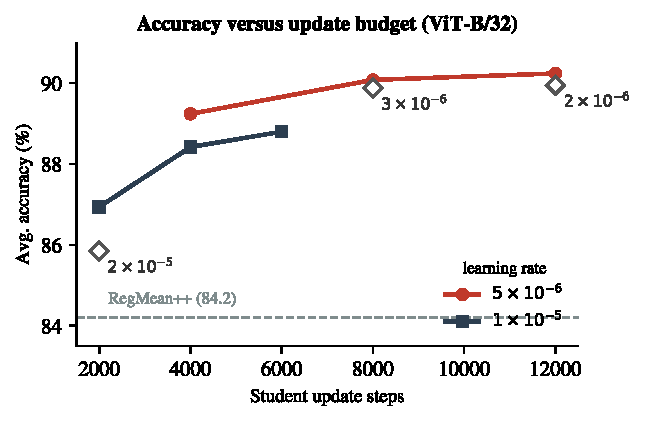
\includegraphics[width=0.94\columnwidth]{fig_lr.pdf}
\caption{Convergence and learning-rate sensitivity on ViT-B/32. Accuracy rises with the
reported step budget and plateaus for the selected rate.}
\label{fig:lr}
\end{figure}

\begin{table}[tb]
\centering
{\small
\begin{tabular*}{\columnwidth}{@{\extracolsep{\fill}}lrrr}
\toprule
Point & Updates & Accuracy & Increment \\
\midrule
RegMean++ & closed form & 84.2 & -- \\
\method & 4k & 89.2 & $+5.0$ vs. RM++ \\
\method & 8k & 90.1 & $+0.9$ vs. 4k \\
\method & 12k & 90.2 & $+0.1$ vs. 8k \\
\bottomrule
\end{tabular*}
}
\caption{Existing ViT-B/32 operating points at the selected learning rate. The table
uses no interpolated wall-clock values: only the 12k endpoint was separately measured at about 35 minutes.}
\label{tab:step-increments-app}
\end{table}

The curve supplies a qualitative, not parametric, test of Corollary~\ref{cor:break-even-formal}.
The first recorded selected-rate point is already above RegMean++, and the reported increments shrink from $5.0$ points at 4k updates to $0.9$ over the next 4k and $0.1$ over the final 4k.
Because accuracy is not the same as $F$ and the intermediate wall-clock was not recorded, these values should not be used to estimate $\mu$, $L$, or a numerical functional break-even time.

\subsection{Refinement from different initializations}
\label{app:refiner}
Table~\ref{tab:refiner} asks whether the endpoint depends on where refinement starts by running the same 8,000-update procedure from a task-arithmetic point, from the RegMean++ solution, and from the pre-trained weights.
Task-arithmetic and RegMean++ starts converge to essentially the same accuracy ($90.1$) despite beginning $16.6$ points apart ($67.6$ vs.\ $84.2$), so in this setting the closed-form solution offers no lasting advantage as an initializer---it only shortens the early transient.
The pre-trained start settles lower ($88.4$), which we read as a weaker basin rather than evidence of global convergence; the experiment does not establish initialization independence in general.

\begin{table}[tb]
\centering
{\small
\begin{tabular*}{\columnwidth}{@{\extracolsep{\fill}}lrr}
\toprule
Initialization & Initial & After \\
\midrule
Task arithmetic ($\alpha=0.3$) & 67.6 & 90.1 \\
RegMean++ & 84.2 & 90.1 \\
Pre-trained ($\alpha=0$) & -- & 88.4 \\
\bottomrule
\end{tabular*}
}
\caption{ViT-B/32 after 8,000 updates from three initializations. Similar endpoints from
task arithmetic and RegMean++ show weak initialization dependence in this setting; they do not prove global convergence or initialization independence in general.}
\label{tab:refiner}
\end{table}

\subsection{Matched unique-example budget}
\label{app:sample-budget}
Table~\ref{tab:sample-budget} and Figure~\ref{fig:dataeff} control for data rather than compute: both methods are given the same number $N$ of distinct unlabeled examples per task, and only the number of distinct examples---not the number of updates or teacher queries---is held equal.
The two methods cross over near $N=256$: below it the single closed-form fit of RegMean++ is the better use of very few examples, above it \method pulls ahead and keeps improving while RegMean++ plateaus around $84.5$.
The crossover is the data-budget analogue of the compute-budget break-even in the main text---iterative refinement wins once there is enough data for its extra passes to extract signal a one-shot fit leaves on the table---and the gain comes at a real cost, since \method reuses those examples over many updates.

\begin{table*}[tb]
\centering
{\small
\begin{tabular}{lrrrrrr}
\toprule
Distinct samples per task & 64 & 128 & 256 & 512 & 1024 & Full-split sampling \\
\midrule
\method, fixed subset & 81.3 & 83.5 & 86.1 & 87.7 & 88.5 & 90.1 \\
RegMean++, matched subset & 83.3 & 83.9 & 84.4 & 84.3 & 84.5 & -- \\
\bottomrule
\end{tabular}
}
\caption{ViT-B/32 accuracy versus the number of distinct unlabeled examples per task.
At $N=256$ and above, \method is more accurate, but it reuses those examples over many updates and therefore consumes more compute and sample exposures.}
\label{tab:sample-budget}
\end{table*}

\begin{figure}[tb]
\centering
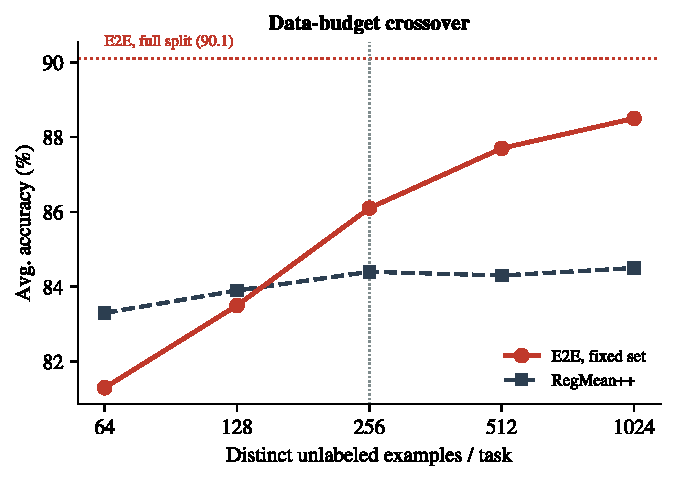
\includegraphics[width=0.94\columnwidth]{fig_dataeff.pdf}
\caption{Matched unique-example comparison. ``Full-split sampling'' repeatedly
reshuffles each finite training split; it should not be interpreted as infinitely many unique samples.}
\label{fig:dataeff}
\end{figure}

\subsection{Residual analysis details}
\label{app:residual-details}
The post-hoc diagnostic records expert-relative hidden-state residuals after each block and the final normalized representation residual.
Summed layer-wise residuals are $2.46$ for RegMean++ and $2.11$ for \method, whereas final residuals are $0.55$ and $0.23$.
Injecting random perturbations at block outputs gives average downstream sensitivity below one in this particular experiment.
We therefore do not use worst-case depth amplification as the explanation.
The evidence is instead consistent with anisotropic downstream geometry and cross-layer interaction, as characterized by Theorems~\ref{thm:exact-gap} and~\ref{thm:cross-layer-gap}.

\subsection{Pairwise task-vector probe}
\label{app:intfprobe}
Table~\ref{tab:intfprobe} tests the common intuition that task-vector geometry predicts how hard a subset is to merge, by pairing each of four fixed subsets with its mean pairwise absolute task-vector cosine.
The two quantities are unrelated over these points (Spearman $\rho=0$): the Digit subset has by far the largest cosine ($0.054$) yet the \emph{smallest} \method--RegMean++ gap ($2.0$), while the Natural subset has a small cosine ($0.026$) but the largest gap ($3.2$).
We read this as evidence against a simple ``cosine interference'' explanation of the merging gap and in favor of the geometric account in the theory section, while noting that four points are too few for a causal conclusion.

\begin{table*}[tb]
\centering
{\small
\begin{tabular}{llrrrrr}
\toprule
Subset & Tasks & Task Arith. & RegMean++ & \method & Gap & Mean $|\cos|$ \\
\midrule
Natural & SUN, Cars, RESISC, EuroSAT & 77.5 & 83.4 & 86.6 & 3.2 & 0.026 \\
Mixed-2 & SVHN, EuroSAT, DTD, Cars & 74.5 & 85.7 & 88.3 & 2.7 & 0.016 \\
Digit & MNIST, SVHN, GTSRB, DTD & 80.5 & 91.7 & 93.8 & 2.0 & 0.054 \\
Mixed-1 & MNIST, GTSRB, RESISC, SUN & 80.1 & 90.3 & 91.9 & 1.7 & 0.026 \\
\bottomrule
\end{tabular}
}
\caption{Four fixed-size ViT-B/32 subsets. Mean pairwise absolute task-vector cosine does
not predict the \method--RegMean++ gap over these four points (reported Spearman $\rho=0$).
The sample is too small for a strong causal conclusion.}
\label{tab:intfprobe}
\end{table*}

\subsection{Block-wise memory--accuracy trade-off}
\label{app:blockwise}
Table~\ref{tab:blockwise} and Figure~\ref{fig:blockwise-main} trace how accuracy varies with the block group size, which is the knob that sets peak activation memory: refining one block at a time caches the fewest activations, refining all twelve jointly caches the most.
Accuracy rises smoothly with group size---from $85.3$ at a single block to $89.8$ for the full-encoder pass---because larger groups retain more of the cross-block coupling that Theorem~\ref{thm:cross-layer-gap} identifies as the source of the closed-form gap; even the smallest, cheapest group already clears RegMean++ ($84.2$).
The curve therefore exposes a tunable operating range rather than a single point: memory can be cut by roughly a third (from $5.4$ to $3.7$ GB on ViT-B/32) at a few points of accuracy, which is the trade-off a memory-constrained user actually faces.

\begin{table*}[tb]
\centering
{\small
\begin{tabular}{lrrrrrrr}
\toprule
Group size & 1 & 2 & 3 & 4 & 6 & 12 (all blocks) & RegMean++ \\
\midrule
Accuracy & 85.3 & 87.4 & 88.4 & 88.9 & 89.2 & 89.8 & 84.2 \\
Peak memory (GB) & 3.7 & 3.9 & 4.0 & 4.2 & 4.5 & 5.4 & -- \\
\bottomrule
\end{tabular}
}
\caption{ViT-B/32 block-wise refinement under the reported total-compute protocol. The
canonical full-encoder run additionally tunes the embedding and projection and reaches 90.2.}
\label{tab:blockwise}
\end{table*}
\begin{figure*}[tb]
\centering
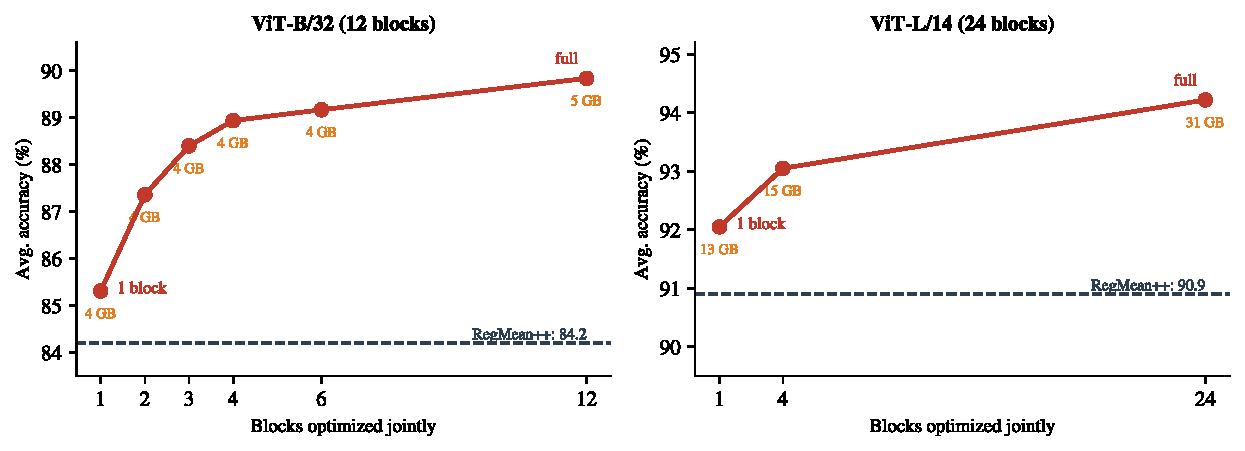
\includegraphics[width=0.83\textwidth]{fig_blockwise.pdf}
\caption{Block-wise accuracy--memory trade-off. Larger groups retain more cross-block
coupling.
On ViT-L/14, a single-block configuration uses about $13$ GB instead of $31$ GB and reaches $92.0\%$ when each block receives the reported adequate update budget; matched-total-compute and caching details are in Appendix~\ref{app:blockwise}.}
\label{fig:blockwise-main}
\end{figure*}





On ViT-L/14, single-block, four-block, and full block-wise runs obtain 92.0, 93.0, and 94.2, with peak activation memory of approximately 13.3, 15.4, and 30.9 GB.
Under a strictly matched total-step budget, the single-block setting is compute starved and reaches about 90.4.
This distinction should be retained when interpreting the figure.

\subsection{Distillation target controls}
\label{app:distillation-control}
Table~\ref{tab:distillation-control} isolates the effect of the distillation target by holding the harness fixed and stepping from the closed-form baseline through logit distillation (with and without a SAM control) to representation matching.
Reading the rows in order separates two contributions: moving from the closed-form fit to any end-to-end objective already recovers most of the gap ($84.2\!\to\!87.9$), and then switching the target from logits to representations adds a further consistent gain ($88.0\!\to\!90.2$ at the matched task-arithmetic init) that the SAM control on logits ($89.1$) does not close.
This ordering is the controlled, same-init version of the ablation conclusion: the representation target, not the choice of initializer or a sharpness regularizer, is what carries the method past logit-based distillation.

\begin{table*}[tb]
\centering
{\small
\begin{tabular}{lllr}
\toprule
Method & Initialization & Target & Accuracy \\
\midrule
RegMean++ & -- & layer regression & 84.2 \\
Logit distillation & pre-trained & KL logits & 87.9 \\
Logit distillation & task arithmetic & KL logits & 88.0 \\
Logit+SAM control & task arithmetic & KL logits+SAM & 89.1 \\
Representation matching & pre-trained & representation & 89.5 \\
\method & task arithmetic & representation & 90.2 \\
\bottomrule
\end{tabular}
}
\caption{ViT-B/32 target and initialization controls. The logit+SAM row is an in-harness
control with a sweep over $\rho\in\{0.02,0.05,0.10\}$; it is not an official SAMerging reproduction.}
\label{tab:distillation-control}
\end{table*}

The best logit+SAM control reaches 89.1 on ViT-B/32.
On ViT-L/14, the corresponding logit and logit+SAM values are 92.4 and 92.9, below representation matching at 94.3.
These results support the target-coverage prediction within the supplied experiments, but they do not replace a direct run of the released SAMerging implementation.

\subsection{From closed-form to end-to-end: a metric-fidelity ladder}
\label{app:gnladder}
The two regimes studied in this paper are not a binary choice but the two ends of a continuum in how faithfully a method models the same local objective, and a single intermediate point makes this explicit.
Consider refining a merge by a damped Gauss--Newton step $\delta^\star=\arg\min_\delta \tfrac12\,\delta^\top(M(\theta)+\lambda I)\delta-b^\top\delta$, with the parameter-space Gauss--Newton matrix $M(\theta)=\sum_a\pi_a\,\mathbb{E}[\mathbf{J}_a^\top \mathbf{J}_a]$ and $b=\sum_a\pi_a\,\mathbb{E}[\mathbf{J}_a^\top r_a]$, updating $\theta\!\leftarrow\!\theta+\delta^\star$ and re-linearizing for a few steps (call this \emph{GN-Merge}).
We solve it \emph{matrix-free} by conjugate gradient---each product $M(\theta)v$ is one Jacobian--vector and one vector--Jacobian product through the encoder, so the $|\theta|\times|\theta|$ matrix is never formed---so GN-Merge runs without any Adam/SGD training loop, though it is not gradient-free, since CG still needs automatic-differentiation products.
RegMean is exactly the isotropic, per-layer truncation of this step, and the part it discards is the anisotropy and cross-layer coupling of $M(\theta)$ that Theorem~\ref{thm:cross-layer-gap} identifies.

\begin{table}[!ht]
\centering
\resizebox{\columnwidth}{!}{%
\begin{tabular}{lccc}
\toprule
Method & Metric & Training loop? & Avg.\ acc.\ (\%) \\
\midrule
Task arithmetic & -- & no & $67.6$ \\
Fisher merging & diagonal & no & $70.3$ \\
RegMean++ & per-layer, isotropic & no & $84.2$ \\
\quad GN-Merge (damped, matrix-free) & full $M(\theta)$ & \textbf{no} & $\mathbf{86.9}$ \\
\textbf{\method} & full, re-evaluated & yes & $\mathbf{90.2}$ \\
\bottomrule
\end{tabular}}
\caption{Increasing the fidelity of the local functional metric on ViT-B/32 (eight tasks).
Each row uses the same unlabeled calibration inputs; only the fidelity of the metric, and
hence the solver, changes. The two end rows do not share an identical data exposure and
optimization budget, so the increments are indicative, not an exact attribution.}
\label{tab:gnladder-app}
\end{table}

Table~\ref{tab:gnladder-app} reads as one continuous ladder of metric fidelity rather than two isolated methods.
Restoring only the anisotropy and cross-layer coupling that RegMean++ truncates---a single matrix-free step, still with no training loop---already lifts accuracy from $84.2$ to $86.9$, an in-place experimental confirmation of Theorem~\ref{thm:cross-layer-gap}; the same pattern holds on ViT-L/14, where GN-Merge reaches $91.9$ against RegMean++'s $90.9$ (full \method: $94.3$).
The one-shot step then saturates below full \method ($90.2$) because a single linearization is exact only to first order in the update, and the nonlinear remainder it drops is largest precisely in the interference-prone regime; recovering it needs the repeated re-linearization that end-to-end refinement performs.
Two caveats travel with this reading: the $86.9\!\to\!90.2$ increment mixes a change of solver with a change of data exposure and compute, so it is directional rather than an exact measure of the nonlinear contribution; and although $M(\theta)$ can be probed spectrally matrix-free, that ratio is confounded by the low rank of $M$, so we do not use it as evidence of anisotropy---the load-bearing evidence is the direct decoupling measurement of Appendix~\ref{app:residual-details}.

\subsection{Preliminary Flan-T5 GLUE probe}
\label{app:nlp}

{\centering {\small
\begin{tabular}{lrr}
\toprule
Method & Seven-task average & MNLI \\
\midrule
Task arithmetic & 79.0 & 57.8 \\
TIES & 80.2 & 65.0 \\
RegMean, closed form & \textbf{83.0} & \textbf{82.1} \\
\method, output KL & 81.9 & 81.0 \\
\bottomrule
\end{tabular}
} \captionof{table}{Preliminary Flan-T5-base GLUE probe.
STS-B is excluded because it is a regression task.
RegMean and the gradient variant use different functional targets, so their difference is not a like-for-like solver comparison.}
\label{tab:nlp}
\par}

Both functional methods exceed the reported weight-space baselines, but the gradient variant does not outperform closed-form RegMean.
The result supports only the limited claim that function-aware merging extends beyond CLIP; it does not establish general superiority of end-to-end representation optimization in language models.
\section{Limitations, Scope, and Broader Impact}
\label{app:limitations}

This is a representative rather than exhaustive comparison.
The clean target control is within the iterative family; the closed-form RegMean++ versus full end-to-end comparison simultaneously changes the trajectory, update freedom, solver, sample exposure, and compute, so it measures an overall regime gap rather than one isolated component.

\subsection{Method and data scope}
\method is label-free but not data-free.
It requires task-specific unlabeled inputs and teacher queries, reuses examples over many updates, and stores or loads the experts.
Teacher storage grows with the number of tasks.
The optimization is a one-time offline cost, but it is materially higher than task-vector and closed-form regression methods.
The block-wise variant reduces activation memory, not the need for teacher information.

All principal experiments merge experts sharing one pre-trained checkpoint, architecture, and representation interface.
Merging independently pre-trained or heterogeneous models is outside the theory and experiments.
The CLIP setting is especially compatible with a shared representation objective because tasks use distinct fixed text-prototype heads.
The preliminary Flan-T5 experiment is not sufficient evidence for decoder-only, generative, or multimodal systems.

\subsection{Theoretical scope}
The Bayes decomposition, frame theorem, and local quadratic gap are exact under their stated mathematical objects.
Their connection to a deep nonlinear merger is local: $Q$ is a damped first-order residual model, and the nonlinear remainder can be large far from the reference point.
The theory does not prove that AdamW reaches a global optimum, that the approximation gap grows monotonically with task count, or that final residual universally ranks all methods.

The RegMean result is deliberately narrow.
RegMean is the exact minimizer of the defined expert-centered, one-layer, first-order, isotropic surrogate.
It is not claimed to be a stationary point of the original nonlinear objective.
RegMean++ changes the activation trajectory and may capture dependencies not represented by the simplest RegMean formula; we use the surrogate analysis to identify omitted structure, not to provide a complete formal model of every implementation detail.

\subsection{Experimental gaps}
The supplied experiments do not directly run the released SAMerging implementation, FeatCal, or Output-Space Projection under the same harness.
The in-harness logit+SAM row is only a controlled target/optimizer baseline.
ViT-B/16 is reported from one run, and not every ablation has multi-seed uncertainty.
The residual diagnostic is post hoc and covers three principal methods; a broader method-level correlation analysis would be needed before using it as a universal unlabeled predictor.

The task-count and backbone trends are consistent with greater consolidation stress, but they do not isolate a single causal interference quantity.
The four-subset task-vector probe is a transparent null result rather than evidence for the proposed mechanism.
Similarly, near-expert recovery is consistent with low irreducible teacher conflict but does not estimate the Bayes conflict term.

\subsection{Positioning as model merging}
The deployment output is one shared encoder with the original architecture and no learned router or task-specific trainable module.
The benchmark still selects a fixed task head.
Algorithmically, \method is a specialized form of multi-teacher representation distillation initialized from a weight-space merge.
Its contribution is not the use of teachers or gradients by itself, but the characterization of the functional target and the approximation gaps of common merger families.

\subsection{Broader impact}
Merging can reduce the storage and serving cost of many specialized models, but it also inherits their biases, errors, and unsafe behaviors.
A merged model may conceal worst-task degradation behind a strong average, so practitioners should audit every task and relevant subgroup.
Because the method consumes unlabeled task inputs, data governance and privacy obligations remain; absence of labels does not imply absence of sensitive information.

\bibliography{references}
\end{document}
